\documentclass[1p]{elsarticle_modified}
%\bibliographystyle{elsarticle-num}

%\usepackage[colorlinks]{hyperref}
%\usepackage{abbrmath_seonhwa} %\Abb, \Ascr, \Acal ,\Abf, \Afrak
\usepackage{amsfonts}
\usepackage{amssymb}
\usepackage{amsmath}
\usepackage{amsthm}
\usepackage{scalefnt}
\usepackage{amsbsy}
\usepackage{kotex}
\usepackage{caption}
\usepackage{subfig}
\usepackage{color}
\usepackage{graphicx}
\usepackage{xcolor} %% white, black, red, green, blue, cyan, magenta, yellow
\usepackage{float}
\usepackage{setspace}
\usepackage{hyperref}

\usepackage{tikz}
\usetikzlibrary{arrows}

\usepackage{multirow}
\usepackage{array} % fixed length table
\usepackage{hhline}

%%%%%%%%%%%%%%%%%%%%%
\makeatletter
\renewcommand*\env@matrix[1][\arraystretch]{%
	\edef\arraystretch{#1}%
	\hskip -\arraycolsep
	\let\@ifnextchar\new@ifnextchar
	\array{*\c@MaxMatrixCols c}}
\makeatother %https://tex.stackexchange.com/questions/14071/how-can-i-increase-the-line-spacing-in-a-matrix
%%%%%%%%%%%%%%%

\usepackage[normalem]{ulem}

\newcommand{\msout}[1]{\ifmmode\text{\sout{\ensuremath{#1}}}\else\sout{#1}\fi}
%SOURCE: \msout is \stkout macro in https://tex.stackexchange.com/questions/20609/strikeout-in-math-mode

\newcommand{\cancel}[1]{
	\ifmmode
	{\color{red}\msout{#1}}
	\else
	{\color{red}\sout{#1}}
	\fi
}

\newcommand{\add}[1]{
	{\color{blue}\uwave{#1}}
}

\newcommand{\replace}[2]{
	\ifmmode
	{\color{red}\msout{#1}}{\color{blue}\uwave{#2}}
	\else
	{\color{red}\sout{#1}}{\color{blue}\uwave{#2}}
	\fi
}

\newcommand{\Sol}{\mathcal{S}} %segment
\newcommand{\D}{D} %diagram
\newcommand{\A}{\mathcal{A}} %arc


%%%%%%%%%%%%%%%%%%%%%%%%%%%%%5 test

\def\sl{\operatorname{\textup{SL}}(2,\Cbb)}
\def\psl{\operatorname{\textup{PSL}}(2,\Cbb)}
\def\quan{\mkern 1mu \triangleright \mkern 1mu}

\theoremstyle{definition}
\newtheorem{thm}{Theorem}[section]
\newtheorem{prop}[thm]{Proposition}
\newtheorem{lem}[thm]{Lemma}
\newtheorem{ques}[thm]{Question}
\newtheorem{cor}[thm]{Corollary}
\newtheorem{defn}[thm]{Definition}
\newtheorem{exam}[thm]{Example}
\newtheorem{rmk}[thm]{Remark}
\newtheorem{alg}[thm]{Algorithm}

\newcommand{\I}{\sqrt{-1}}
\begin{document}

%\begin{frontmatter}
%
%\title{Boundary parabolic representations of knots up to 8 crossings}
%
%%% Group authors per affiliation:
%\author{Yunhi Cho} 
%\address{Department of Mathematics, University of Seoul, Seoul, Korea}
%\ead{yhcho@uos.ac.kr}
%
%
%\author{Seonhwa Kim} %\fnref{s_kim}}
%\address{Center for Geometry and Physics, Institute for Basic Science, Pohang, 37673, Korea}
%\ead{ryeona17@ibs.re.kr}
%
%\author{Hyuk Kim}
%\address{Department of Mathematical Sciences, Seoul National University, Seoul 08826, Korea}
%\ead{hyukkim@snu.ac.kr}
%
%\author{Seokbeom Yoon}
%\address{Department of Mathematical Sciences, Seoul National University, Seoul, 08826,  Korea}
%\ead{sbyoon15@snu.ac.kr}
%
%\begin{abstract}
%We find all boundary parabolic representation of knots up to 8 crossings.
%
%\end{abstract}
%\begin{keyword}
%    \MSC[2010] 57M25 
%\end{keyword}
%
%\end{frontmatter}

%\linenumbers
%\tableofcontents
%
\newcommand\colored[1]{\textcolor{white}{\rule[-0.35ex]{0.8em}{1.4ex}}\kern-0.8em\color{red} #1}%
%\newcommand\colored[1]{\textcolor{white}{ #1}\kern-2.17ex	\textcolor{white}{ #1}\kern-1.81ex	\textcolor{white}{ #1}\kern-2.15ex\color{red}#1	}

{\Large $\underline{12a_{0487}~(K12a_{0487})}$}

\setlength{\tabcolsep}{10pt}
\renewcommand{\arraystretch}{1.6}
\vspace{1cm}\begin{tabular}{m{100pt}>{\centering\arraybackslash}m{274pt}}
\multirow{5}{120pt}{
	\centering
	\includegraphics[width=112pt]{../../../GIT/diagram.site/Diagrams/png/1288_12a_0487.png}\\
\ \ \ A knot diagram\footnotemark}&
\allowdisplaybreaks
\textbf{Linearized knot diagam} \\
\cline{2-2}
 &
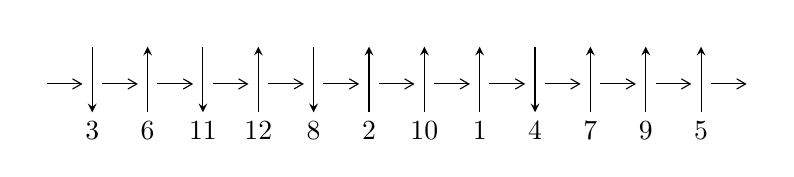
\begin{tikzpicture}[x=20pt, y=17pt]
	% nodes
	\node (C0) at (0, 0) {};
	\node (C1) at (1, 0) {};
	\node (C1U) at (1, +1) {};
	\node (C1D) at (1, -1) {3};

	\node (C2) at (2, 0) {};
	\node (C2U) at (2, +1) {};
	\node (C2D) at (2, -1) {6};

	\node (C3) at (3, 0) {};
	\node (C3U) at (3, +1) {};
	\node (C3D) at (3, -1) {11};

	\node (C4) at (4, 0) {};
	\node (C4U) at (4, +1) {};
	\node (C4D) at (4, -1) {12};

	\node (C5) at (5, 0) {};
	\node (C5U) at (5, +1) {};
	\node (C5D) at (5, -1) {8};

	\node (C6) at (6, 0) {};
	\node (C6U) at (6, +1) {};
	\node (C6D) at (6, -1) {2};

	\node (C7) at (7, 0) {};
	\node (C7U) at (7, +1) {};
	\node (C7D) at (7, -1) {10};

	\node (C8) at (8, 0) {};
	\node (C8U) at (8, +1) {};
	\node (C8D) at (8, -1) {1};

	\node (C9) at (9, 0) {};
	\node (C9U) at (9, +1) {};
	\node (C9D) at (9, -1) {4};

	\node (C10) at (10, 0) {};
	\node (C10U) at (10, +1) {};
	\node (C10D) at (10, -1) {7};

	\node (C11) at (11, 0) {};
	\node (C11U) at (11, +1) {};
	\node (C11D) at (11, -1) {9};

	\node (C12) at (12, 0) {};
	\node (C12U) at (12, +1) {};
	\node (C12D) at (12, -1) {5};
	\node (C13) at (13, 0) {};

	% arrows
	\draw[->,>={angle 60}]
	(C0) edge (C1) (C1) edge (C2) (C2) edge (C3) (C3) edge (C4) (C4) edge (C5) (C5) edge (C6) (C6) edge (C7) (C7) edge (C8) (C8) edge (C9) (C9) edge (C10) (C10) edge (C11) (C11) edge (C12) (C12) edge (C13) ;	\draw[->,>=stealth]
	(C1U) edge (C1D) (C2D) edge (C2U) (C3U) edge (C3D) (C4D) edge (C4U) (C5U) edge (C5D) (C6D) edge (C6U) (C7D) edge (C7U) (C8D) edge (C8U) (C9U) edge (C9D) (C10D) edge (C10U) (C11D) edge (C11U) (C12D) edge (C12U) ;
	\end{tikzpicture} \\
\hhline{~~} \\& 
\textbf{Solving Sequence} \\ \cline{2-2} 
 &
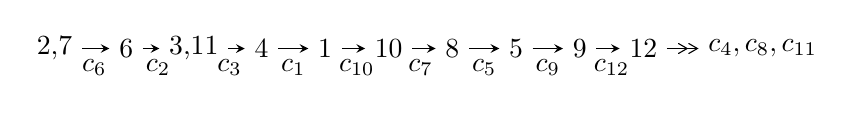
\begin{tikzpicture}[x=23pt, y=7pt]
	% node
	\node (A0) at (-1/8, 0) {2,7};
	\node (A1) at (1, 0) {6};
	\node (A2) at (33/16, 0) {3,11};
	\node (A3) at (25/8, 0) {4};
	\node (A4) at (33/8, 0) {1};
	\node (A5) at (41/8, 0) {10};
	\node (A6) at (49/8, 0) {8};
	\node (A7) at (57/8, 0) {5};
	\node (A8) at (65/8, 0) {9};
	\node (A9) at (73/8, 0) {12};
	\node (C1) at (1/2, -1) {$c_{6}$};
	\node (C2) at (3/2, -1) {$c_{2}$};
	\node (C3) at (21/8, -1) {$c_{3}$};
	\node (C4) at (29/8, -1) {$c_{1}$};
	\node (C5) at (37/8, -1) {$c_{10}$};
	\node (C6) at (45/8, -1) {$c_{7}$};
	\node (C7) at (53/8, -1) {$c_{5}$};
	\node (C8) at (61/8, -1) {$c_{9}$};
	\node (C9) at (69/8, -1) {$c_{12}$};
	\node (A10) at (11, 0) {$c_{4},c_{8},c_{11}$};

	% edge
	\draw[->,>=stealth]	
	(A0) edge (A1) (A1) edge (A2) (A2) edge (A3) (A3) edge (A4) (A4) edge (A5) (A5) edge (A6) (A6) edge (A7) (A7) edge (A8) (A8) edge (A9) ;
	\draw[->>,>={angle 60}]	
	(A9) edge (A10);
\end{tikzpicture} \\ 

\end{tabular} \\

\footnotetext{
The image of knot diagram is generated by the software ``\textbf{Draw programme}" developed by Andrew Bartholomew(\url{http://www.layer8.co.uk/maths/draw/index.htm\#Running-draw}), where we modified some parts for our purpose(\url{https://github.com/CATsTAILs/LinksPainter}).
}\phantom \\ \newline 
\centering \textbf{Ideals for irreducible components\footnotemark of $X_{\text{par}}$} 
 
\begin{align*}
I^u_{1}&=\langle 
6.97834\times10^{541} u^{174}+6.18922\times10^{542} u^{173}+\cdots+5.84381\times10^{542} b+4.55462\times10^{545},\\
\phantom{I^u_{1}}&\phantom{= \langle  }3.74109\times10^{545} u^{174}+1.30601\times10^{546} u^{173}+\cdots+6.52753\times10^{545} a+4.73645\times10^{547},\\
\phantom{I^u_{1}}&\phantom{= \langle  }u^{175}+4 u^{174}+\cdots+6175 u+1117\rangle \\
I^u_{2}&=\langle 
8832633158 u^{43}+28505051997 u^{42}+\cdots+4990744411 b+36995583025,\\
\phantom{I^u_{2}}&\phantom{= \langle  }53295260397 u^{43}-140240440915 u^{42}+\cdots+4990744411 a-80983955218,\\
\phantom{I^u_{2}}&\phantom{= \langle  }u^{44}- u^{43}+\cdots-5 u+1\rangle \\
\\
\end{align*}
\raggedright * 2 irreducible components of $\dim_{\mathbb{C}}=0$, with total 219 representations.\\
\footnotetext{All coefficients of polynomials are rational numbers. But the coefficients are sometimes approximated in decimal forms when there is not enough margin.}
\newpage
\renewcommand{\arraystretch}{1}
\centering \section*{I. $I^u_{1}= \langle 6.98\times10^{541} u^{174}+6.19\times10^{542} u^{173}+\cdots+5.84\times10^{542} b+4.55\times10^{545},\;3.74\times10^{545} u^{174}+1.31\times10^{546} u^{173}+\cdots+6.53\times10^{545} a+4.74\times10^{547},\;u^{175}+4 u^{174}+\cdots+6175 u+1117 \rangle$}
\flushleft \textbf{(i) Arc colorings}\\
\begin{tabular}{m{7pt} m{180pt} m{7pt} m{180pt} }
\flushright $a_{2}=$&$\begin{pmatrix}0\\u\end{pmatrix}$ \\
\flushright $a_{7}=$&$\begin{pmatrix}1\\0\end{pmatrix}$ \\
\flushright $a_{6}=$&$\begin{pmatrix}1\\u^2\end{pmatrix}$ \\
\flushright $a_{3}=$&$\begin{pmatrix}u\\u^3+u\end{pmatrix}$ \\
\flushright $a_{11}=$&$\begin{pmatrix}-0.573125 u^{174}-2.00077 u^{173}+\cdots-1079.69 u-72.5611\\-0.119414 u^{174}-1.05911 u^{173}+\cdots-3832.66 u-779.393\end{pmatrix}$ \\
\flushright $a_{4}=$&$\begin{pmatrix}0.669635 u^{174}+0.835488 u^{173}+\cdots-6116.01 u-1455.53\\-0.256227 u^{174}-0.356799 u^{173}+\cdots+2129.74 u+508.045\end{pmatrix}$ \\
\flushright $a_{1}=$&$\begin{pmatrix}u^3\\u^5+u^3+u\end{pmatrix}$ \\
\flushright $a_{10}=$&$\begin{pmatrix}-0.453711 u^{174}-0.941658 u^{173}+\cdots+2752.96 u+706.832\\-0.119414 u^{174}-1.05911 u^{173}+\cdots-3832.66 u-779.393\end{pmatrix}$ \\
\flushright $a_{8}=$&$\begin{pmatrix}-2.07547 u^{174}-7.00149 u^{173}+\cdots-3353.22 u-202.885\\0.0526862 u^{174}-0.663567 u^{173}+\cdots-4427.74 u-936.746\end{pmatrix}$ \\
\flushright $a_{5}=$&$\begin{pmatrix}0.104480 u^{174}+1.55732 u^{173}+\cdots+5981.79 u+1247.39\\0.0420972 u^{174}-0.484376 u^{173}+\cdots-2892.27 u-619.913\end{pmatrix}$ \\
\flushright $a_{9}=$&$\begin{pmatrix}-2.09026 u^{174}-7.90330 u^{173}+\cdots-8049.25 u-1190.52\\-0.0104941 u^{174}-0.486964 u^{173}+\cdots-2360.15 u-486.146\end{pmatrix}$ \\
\flushright $a_{12}=$&$\begin{pmatrix}1.05839 u^{174}+5.35345 u^{173}+\cdots+11562.0 u+2160.82\\-0.305282 u^{174}-1.96470 u^{173}+\cdots-5457.81 u-1056.61\end{pmatrix}$\\&\end{tabular}
\flushleft \textbf{(ii) Obstruction class $= -1$}\\~\\
\flushleft \textbf{(iii) Cusp Shapes $= -1.32452 u^{174}-4.02580 u^{173}+\cdots+31.4211 u+283.875$}\\~\\
\newpage\renewcommand{\arraystretch}{1}
\flushleft \textbf{(iv) u-Polynomials at the component}\newline \\
\begin{tabular}{m{50pt}|m{274pt}}
Crossings & \hspace{64pt}u-Polynomials at each crossing \\
\hline $$\begin{aligned}c_{1}\end{aligned}$$&$\begin{aligned}
&u^{175}+84 u^{174}+\cdots-21510473 u-1247689
\end{aligned}$\\
\hline $$\begin{aligned}c_{2},c_{6}\end{aligned}$$&$\begin{aligned}
&u^{175}-4 u^{174}+\cdots+6175 u-1117
\end{aligned}$\\
\hline $$\begin{aligned}c_{3}\end{aligned}$$&$\begin{aligned}
&u^{175}+5 u^{174}+\cdots-200903543 u-14492227
\end{aligned}$\\
\hline $$\begin{aligned}c_{4},c_{12}\end{aligned}$$&$\begin{aligned}
&u^{175}+u^{174}+\cdots+38 u-1
\end{aligned}$\\
\hline $$\begin{aligned}c_{5}\end{aligned}$$&$\begin{aligned}
&u^{175}-9 u^{174}+\cdots+1244051648 u-87632999
\end{aligned}$\\
\hline $$\begin{aligned}c_{7},c_{10}\end{aligned}$$&$\begin{aligned}
&u^{175}-14 u^{174}+\cdots+444875 u-24751
\end{aligned}$\\
\hline $$\begin{aligned}c_{8}\end{aligned}$$&$\begin{aligned}
&u^{175}-3 u^{174}+\cdots-3228 u-745
\end{aligned}$\\
\hline $$\begin{aligned}c_{9}\end{aligned}$$&$\begin{aligned}
&u^{175}- u^{174}+\cdots-1852932 u-499117
\end{aligned}$\\
\hline $$\begin{aligned}c_{11}\end{aligned}$$&$\begin{aligned}
&u^{175}+13 u^{174}+\cdots-2 u+97
\end{aligned}$\\
\hline
\end{tabular}\\~\\
\newpage\renewcommand{\arraystretch}{1}
\flushleft \textbf{(v) Riley Polynomials at the component}\newline \\
\begin{tabular}{m{50pt}|m{274pt}}
Crossings & \hspace{64pt}Riley Polynomials at each crossing \\
\hline $$\begin{aligned}c_{1}\end{aligned}$$&$\begin{aligned}
&y^{175}+28 y^{174}+\cdots-85299694583841 y-1556727840721
\end{aligned}$\\
\hline $$\begin{aligned}c_{2},c_{6}\end{aligned}$$&$\begin{aligned}
&y^{175}+84 y^{174}+\cdots-21510473 y-1247689
\end{aligned}$\\
\hline $$\begin{aligned}c_{3}\end{aligned}$$&$\begin{aligned}
&y^{175}-37 y^{174}+\cdots+10887680210935327 y-210024643419529
\end{aligned}$\\
\hline $$\begin{aligned}c_{4},c_{12}\end{aligned}$$&$\begin{aligned}
&y^{175}-127 y^{174}+\cdots-180 y-1
\end{aligned}$\\
\hline $$\begin{aligned}c_{5}\end{aligned}$$&$\begin{aligned}
&y^{175}+27 y^{174}+\cdots+136692045245606196 y-7679542513734001
\end{aligned}$\\
\hline $$\begin{aligned}c_{7},c_{10}\end{aligned}$$&$\begin{aligned}
&y^{175}+94 y^{174}+\cdots-17564282207 y-612612001
\end{aligned}$\\
\hline $$\begin{aligned}c_{8}\end{aligned}$$&$\begin{aligned}
&y^{175}-29 y^{174}+\cdots+14232894 y-555025
\end{aligned}$\\
\hline $$\begin{aligned}c_{9}\end{aligned}$$&$\begin{aligned}
&y^{175}+29 y^{174}+\cdots-22256433571302 y-249117779689
\end{aligned}$\\
\hline $$\begin{aligned}c_{11}\end{aligned}$$&$\begin{aligned}
&y^{175}-27 y^{174}+\cdots+580452 y-9409
\end{aligned}$\\
\hline
\end{tabular}\\~\\
\newpage\flushleft \textbf{(vi) Complex Volumes and Cusp Shapes}
$$\begin{array}{c|c|c}  
\text{Solutions to }I^u_{1}& \I (\text{vol} + \sqrt{-1}CS) & \text{Cusp shape}\\
 \hline 
\begin{aligned}
u &= \phantom{-}0.325956 + 0.949466 I \\
a &= -2.60340 + 1.92275 I \\
b &= \phantom{-}0.005403 - 0.767784 I\end{aligned}
 & \phantom{-}1.58192 - 4.67301 I & \phantom{-0.000000 } 0 \\ \hline\begin{aligned}
u &= \phantom{-}0.325956 - 0.949466 I \\
a &= -2.60340 - 1.92275 I \\
b &= \phantom{-}0.005403 + 0.767784 I\end{aligned}
 & \phantom{-}1.58192 + 4.67301 I & \phantom{-0.000000 } 0 \\ \hline\begin{aligned}
u &= -0.987821 + 0.189772 I \\
a &= -0.326720 - 0.404313 I \\
b &= -0.347434 - 1.012110 I\end{aligned}
 & -0.65552 + 1.79433 I & \phantom{-0.000000 } 0 \\ \hline\begin{aligned}
u &= -0.987821 - 0.189772 I \\
a &= -0.326720 + 0.404313 I \\
b &= -0.347434 + 1.012110 I\end{aligned}
 & -0.65552 - 1.79433 I & \phantom{-0.000000 } 0 \\ \hline\begin{aligned}
u &= -0.364947 + 0.924553 I \\
a &= -1.54353 - 1.00452 I \\
b &= -0.452814 - 0.602040 I\end{aligned}
 & -2.29353 - 2.27823 I & \phantom{-0.000000 } 0 \\ \hline\begin{aligned}
u &= -0.364947 - 0.924553 I \\
a &= -1.54353 + 1.00452 I \\
b &= -0.452814 + 0.602040 I\end{aligned}
 & -2.29353 + 2.27823 I & \phantom{-0.000000 } 0 \\ \hline\begin{aligned}
u &= -0.813844 + 0.565118 I \\
a &= -0.413123 - 1.262400 I \\
b &= -0.701528 - 1.210640 I\end{aligned}
 & \phantom{-}2.87174 + 4.67293 I & \phantom{-0.000000 } 0 \\ \hline\begin{aligned}
u &= -0.813844 - 0.565118 I \\
a &= -0.413123 + 1.262400 I \\
b &= -0.701528 + 1.210640 I\end{aligned}
 & \phantom{-}2.87174 - 4.67293 I & \phantom{-0.000000 } 0 \\ \hline\begin{aligned}
u &= -0.958683 + 0.245748 I \\
a &= \phantom{-}1.142750 + 0.622428 I \\
b &= \phantom{-}0.609432 + 0.907836 I\end{aligned}
 & \phantom{-}3.30252 + 1.79502 I & \phantom{-0.000000 } 0 \\ \hline\begin{aligned}
u &= -0.958683 - 0.245748 I \\
a &= \phantom{-}1.142750 - 0.622428 I \\
b &= \phantom{-}0.609432 - 0.907836 I\end{aligned}
 & \phantom{-}3.30252 - 1.79502 I & \phantom{-0.000000 } 0\\
 \hline 
 \end{array}$$\newpage$$\begin{array}{c|c|c}  
\text{Solutions to }I^u_{1}& \I (\text{vol} + \sqrt{-1}CS) & \text{Cusp shape}\\
 \hline 
\begin{aligned}
u &= \phantom{-}0.271679 + 0.975980 I \\
a &= -1.59863 + 1.69105 I \\
b &= -0.043481 + 0.141822 I\end{aligned}
 & \phantom{-}1.68466 + 6.98103 I & \phantom{-0.000000 } 0 \\ \hline\begin{aligned}
u &= \phantom{-}0.271679 - 0.975980 I \\
a &= -1.59863 - 1.69105 I \\
b &= -0.043481 - 0.141822 I\end{aligned}
 & \phantom{-}1.68466 - 6.98103 I & \phantom{-0.000000 } 0 \\ \hline\begin{aligned}
u &= -0.249223 + 0.951198 I \\
a &= \phantom{-}0.022733 - 1.350770 I \\
b &= -0.090871 + 1.315720 I\end{aligned}
 & -4.79455 - 2.50479 I & \phantom{-0.000000 } 0 \\ \hline\begin{aligned}
u &= -0.249223 - 0.951198 I \\
a &= \phantom{-}0.022733 + 1.350770 I \\
b &= -0.090871 - 1.315720 I\end{aligned}
 & -4.79455 + 2.50479 I & \phantom{-0.000000 } 0 \\ \hline\begin{aligned}
u &= -0.950176 + 0.364365 I \\
a &= \phantom{-}0.941037 + 0.799797 I \\
b &= \phantom{-}0.670816 + 1.243370 I\end{aligned}
 & \phantom{-}3.1539 + 14.7991 I & \phantom{-0.000000 } 0 \\ \hline\begin{aligned}
u &= -0.950176 - 0.364365 I \\
a &= \phantom{-}0.941037 - 0.799797 I \\
b &= \phantom{-}0.670816 - 1.243370 I\end{aligned}
 & \phantom{-}3.1539 - 14.7991 I & \phantom{-0.000000 } 0 \\ \hline\begin{aligned}
u &= -0.355020 + 0.959098 I \\
a &= -0.194170 + 1.160960 I \\
b &= -0.273227 - 1.323650 I\end{aligned}
 & -5.19352 + 0.07694 I & \phantom{-0.000000 } 0 \\ \hline\begin{aligned}
u &= -0.355020 - 0.959098 I \\
a &= -0.194170 - 1.160960 I \\
b &= -0.273227 + 1.323650 I\end{aligned}
 & -5.19352 - 0.07694 I & \phantom{-0.000000 } 0 \\ \hline\begin{aligned}
u &= \phantom{-}0.407927 + 0.886173 I \\
a &= -0.729651 + 0.787225 I \\
b &= -0.927594 + 1.034960 I\end{aligned}
 & \phantom{-}2.29763 - 1.16801 I & \phantom{-0.000000 } 0 \\ \hline\begin{aligned}
u &= \phantom{-}0.407927 - 0.886173 I \\
a &= -0.729651 - 0.787225 I \\
b &= -0.927594 - 1.034960 I\end{aligned}
 & \phantom{-}2.29763 + 1.16801 I & \phantom{-0.000000 } 0\\
 \hline 
 \end{array}$$\newpage$$\begin{array}{c|c|c}  
\text{Solutions to }I^u_{1}& \I (\text{vol} + \sqrt{-1}CS) & \text{Cusp shape}\\
 \hline 
\begin{aligned}
u &= \phantom{-}0.143310 + 1.014600 I \\
a &= \phantom{-}0.543110 - 0.814198 I \\
b &= -0.230486 + 1.383780 I\end{aligned}
 & -5.13023 - 2.18375 I & \phantom{-0.000000 } 0 \\ \hline\begin{aligned}
u &= \phantom{-}0.143310 - 1.014600 I \\
a &= \phantom{-}0.543110 + 0.814198 I \\
b &= -0.230486 - 1.383780 I\end{aligned}
 & -5.13023 + 2.18375 I & \phantom{-0.000000 } 0 \\ \hline\begin{aligned}
u &= \phantom{-}0.961868 + 0.363103 I \\
a &= \phantom{-}0.933450 - 0.715334 I \\
b &= \phantom{-}0.588144 - 1.160490 I\end{aligned}
 & -1.48419 - 8.82684 I & \phantom{-0.000000 } 0 \\ \hline\begin{aligned}
u &= \phantom{-}0.961868 - 0.363103 I \\
a &= \phantom{-}0.933450 + 0.715334 I \\
b &= \phantom{-}0.588144 + 1.160490 I\end{aligned}
 & -1.48419 + 8.82684 I & \phantom{-0.000000 } 0 \\ \hline\begin{aligned}
u &= \phantom{-}0.414434 + 0.874408 I \\
a &= -1.80192 + 1.45961 I \\
b &= -0.658138 - 1.119250 I\end{aligned}
 & \phantom{-}2.31978 + 4.58023 I & \phantom{-0.000000 } 0 \\ \hline\begin{aligned}
u &= \phantom{-}0.414434 - 0.874408 I \\
a &= -1.80192 - 1.45961 I \\
b &= -0.658138 + 1.119250 I\end{aligned}
 & \phantom{-}2.31978 - 4.58023 I & \phantom{-0.000000 } 0 \\ \hline\begin{aligned}
u &= -0.902569 + 0.345482 I \\
a &= \phantom{-}1.55696 - 0.21348 I \\
b &= \phantom{-}0.665240 - 0.822100 I\end{aligned}
 & \phantom{-}3.57840 - 3.20414 I & \phantom{-0.000000 } 0 \\ \hline\begin{aligned}
u &= -0.902569 - 0.345482 I \\
a &= \phantom{-}1.55696 + 0.21348 I \\
b &= \phantom{-}0.665240 + 0.822100 I\end{aligned}
 & \phantom{-}3.57840 + 3.20414 I & \phantom{-0.000000 } 0 \\ \hline\begin{aligned}
u &= -0.356050 + 0.898168 I \\
a &= -2.25572 - 2.08663 I \\
b &= -0.218914 + 0.896821 I\end{aligned}
 & -2.18994 - 0.67486 I & \phantom{-0.000000 } 0 \\ \hline\begin{aligned}
u &= -0.356050 - 0.898168 I \\
a &= -2.25572 + 2.08663 I \\
b &= -0.218914 - 0.896821 I\end{aligned}
 & -2.18994 + 0.67486 I & \phantom{-0.000000 } 0\\
 \hline 
 \end{array}$$\newpage$$\begin{array}{c|c|c}  
\text{Solutions to }I^u_{1}& \I (\text{vol} + \sqrt{-1}CS) & \text{Cusp shape}\\
 \hline 
\begin{aligned}
u &= \phantom{-}0.680433 + 0.677818 I \\
a &= -0.572994 + 1.149020 I \\
b &= -0.839860 + 0.269339 I\end{aligned}
 & \phantom{-}4.68042 - 0.92261 I & \phantom{-0.000000 } 0 \\ \hline\begin{aligned}
u &= \phantom{-}0.680433 - 0.677818 I \\
a &= -0.572994 - 1.149020 I \\
b &= -0.839860 - 0.269339 I\end{aligned}
 & \phantom{-}4.68042 + 0.92261 I & \phantom{-0.000000 } 0 \\ \hline\begin{aligned}
u &= -0.568795 + 0.764886 I \\
a &= -1.41968 - 1.20891 I \\
b &= -1.273990 + 0.431196 I\end{aligned}
 & \phantom{-}5.45673 - 2.09442 I & \phantom{-0.000000 } 0 \\ \hline\begin{aligned}
u &= -0.568795 - 0.764886 I \\
a &= -1.41968 + 1.20891 I \\
b &= -1.273990 - 0.431196 I\end{aligned}
 & \phantom{-}5.45673 + 2.09442 I & \phantom{-0.000000 } 0 \\ \hline\begin{aligned}
u &= \phantom{-}0.958711 + 0.434750 I \\
a &= -0.255889 + 0.807548 I \\
b &= -0.417655 + 1.259020 I\end{aligned}
 & \phantom{-}0.23870 - 5.12314 I & \phantom{-0.000000 } 0 \\ \hline\begin{aligned}
u &= \phantom{-}0.958711 - 0.434750 I \\
a &= -0.255889 - 0.807548 I \\
b &= -0.417655 - 1.259020 I\end{aligned}
 & \phantom{-}0.23870 + 5.12314 I & \phantom{-0.000000 } 0 \\ \hline\begin{aligned}
u &= -0.518573 + 0.917086 I \\
a &= -1.07979 - 1.09258 I \\
b &= -1.56419 - 0.26869 I\end{aligned}
 & \phantom{-}4.99730 - 2.25058 I & \phantom{-0.000000 } 0 \\ \hline\begin{aligned}
u &= -0.518573 - 0.917086 I \\
a &= -1.07979 + 1.09258 I \\
b &= -1.56419 + 0.26869 I\end{aligned}
 & \phantom{-}4.99730 + 2.25058 I & \phantom{-0.000000 } 0 \\ \hline\begin{aligned}
u &= -0.273045 + 1.019310 I \\
a &= \phantom{-}0.570187 + 0.122249 I \\
b &= \phantom{-}0.303173 + 0.378363 I\end{aligned}
 & -1.17420 - 2.79461 I & \phantom{-0.000000 } 0 \\ \hline\begin{aligned}
u &= -0.273045 - 1.019310 I \\
a &= \phantom{-}0.570187 - 0.122249 I \\
b &= \phantom{-}0.303173 - 0.378363 I\end{aligned}
 & -1.17420 + 2.79461 I & \phantom{-0.000000 } 0\\
 \hline 
 \end{array}$$\newpage$$\begin{array}{c|c|c}  
\text{Solutions to }I^u_{1}& \I (\text{vol} + \sqrt{-1}CS) & \text{Cusp shape}\\
 \hline 
\begin{aligned}
u &= \phantom{-}0.148278 + 1.051400 I \\
a &= \phantom{-}0.608011 - 0.731055 I \\
b &= \phantom{-}0.688728 - 0.200996 I\end{aligned}
 & -3.85938 - 1.61276 I & \phantom{-0.000000 } 0 \\ \hline\begin{aligned}
u &= \phantom{-}0.148278 - 1.051400 I \\
a &= \phantom{-}0.608011 + 0.731055 I \\
b &= \phantom{-}0.688728 + 0.200996 I\end{aligned}
 & -3.85938 + 1.61276 I & \phantom{-0.000000 } 0 \\ \hline\begin{aligned}
u &= -0.155373 + 1.052830 I \\
a &= \phantom{-}0.611196 + 1.200530 I \\
b &= \phantom{-}0.945554 + 0.107943 I\end{aligned}
 & \phantom{-}1.04897 + 6.48994 I & \phantom{-0.000000 } 0 \\ \hline\begin{aligned}
u &= -0.155373 - 1.052830 I \\
a &= \phantom{-}0.611196 - 1.200530 I \\
b &= \phantom{-}0.945554 - 0.107943 I\end{aligned}
 & \phantom{-}1.04897 - 6.48994 I & \phantom{-0.000000 } 0 \\ \hline\begin{aligned}
u &= -0.761759 + 0.541233 I \\
a &= \phantom{-}0.849597 - 0.002654 I \\
b &= \phantom{-}0.399416 + 0.813177 I\end{aligned}
 & \phantom{-}1.31816 - 0.63282 I & \phantom{-0.000000 } 0 \\ \hline\begin{aligned}
u &= -0.761759 - 0.541233 I \\
a &= \phantom{-}0.849597 + 0.002654 I \\
b &= \phantom{-}0.399416 - 0.813177 I\end{aligned}
 & \phantom{-}1.31816 + 0.63282 I & \phantom{-0.000000 } 0 \\ \hline\begin{aligned}
u &= \phantom{-}0.820029 + 0.709079 I \\
a &= \phantom{-}0.910069 + 0.628289 I \\
b &= \phantom{-}0.444111 + 0.577934 I\end{aligned}
 & \phantom{-}6.25198 - 1.81788 I & \phantom{-0.000000 } 0 \\ \hline\begin{aligned}
u &= \phantom{-}0.820029 - 0.709079 I \\
a &= \phantom{-}0.910069 - 0.628289 I \\
b &= \phantom{-}0.444111 - 0.577934 I\end{aligned}
 & \phantom{-}6.25198 + 1.81788 I & \phantom{-0.000000 } 0 \\ \hline\begin{aligned}
u &= \phantom{-}0.322487 + 1.039360 I \\
a &= \phantom{-}0.511525 - 1.204290 I \\
b &= -0.27949 + 1.45121 I\end{aligned}
 & -4.22651 - 3.50011 I & \phantom{-0.000000 } 0 \\ \hline\begin{aligned}
u &= \phantom{-}0.322487 - 1.039360 I \\
a &= \phantom{-}0.511525 + 1.204290 I \\
b &= -0.27949 - 1.45121 I\end{aligned}
 & -4.22651 + 3.50011 I & \phantom{-0.000000 } 0\\
 \hline 
 \end{array}$$\newpage$$\begin{array}{c|c|c}  
\text{Solutions to }I^u_{1}& \I (\text{vol} + \sqrt{-1}CS) & \text{Cusp shape}\\
 \hline 
\begin{aligned}
u &= \phantom{-}0.496814 + 0.970984 I \\
a &= -0.796063 + 1.124390 I \\
b &= -1.278770 + 0.259072 I\end{aligned}
 & \phantom{-}1.41529 + 2.64820 I & \phantom{-0.000000 } 0 \\ \hline\begin{aligned}
u &= \phantom{-}0.496814 - 0.970984 I \\
a &= -0.796063 - 1.124390 I \\
b &= -1.278770 - 0.259072 I\end{aligned}
 & \phantom{-}1.41529 - 2.64820 I & \phantom{-0.000000 } 0 \\ \hline\begin{aligned}
u &= \phantom{-}0.751149 + 0.508223 I \\
a &= \phantom{-}0.749854 + 0.217362 I \\
b &= \phantom{-}0.613536 - 0.689882 I\end{aligned}
 & \phantom{-}6.29900 + 5.67352 I & \phantom{-0.000000 } 0 \\ \hline\begin{aligned}
u &= \phantom{-}0.751149 - 0.508223 I \\
a &= \phantom{-}0.749854 - 0.217362 I \\
b &= \phantom{-}0.613536 + 0.689882 I\end{aligned}
 & \phantom{-}6.29900 - 5.67352 I & \phantom{-0.000000 } 0 \\ \hline\begin{aligned}
u &= -0.426630 + 1.022100 I \\
a &= -0.973462 - 0.343443 I \\
b &= \phantom{-}0.11014 + 1.71170 I\end{aligned}
 & -3.59033 - 7.63415 I & \phantom{-0.000000 } 0 \\ \hline\begin{aligned}
u &= -0.426630 - 1.022100 I \\
a &= -0.973462 + 0.343443 I \\
b &= \phantom{-}0.11014 - 1.71170 I\end{aligned}
 & -3.59033 + 7.63415 I & \phantom{-0.000000 } 0 \\ \hline\begin{aligned}
u &= -0.658238 + 0.588206 I \\
a &= -0.478003 - 0.070068 I \\
b &= -0.426802 + 0.496050 I\end{aligned}
 & \phantom{-}0.68565 - 1.44589 I & \phantom{-0.000000 } 0 \\ \hline\begin{aligned}
u &= -0.658238 - 0.588206 I \\
a &= -0.478003 + 0.070068 I \\
b &= -0.426802 - 0.496050 I\end{aligned}
 & \phantom{-}0.68565 + 1.44589 I & \phantom{-0.000000 } 0 \\ \hline\begin{aligned}
u &= -0.495890 + 1.002680 I \\
a &= -0.60282 - 1.54683 I \\
b &= -1.49918 - 0.22333 I\end{aligned}
 & \phantom{-}4.62733 - 2.83690 I & \phantom{-0.000000 } 0 \\ \hline\begin{aligned}
u &= -0.495890 - 1.002680 I \\
a &= -0.60282 + 1.54683 I \\
b &= -1.49918 + 0.22333 I\end{aligned}
 & \phantom{-}4.62733 + 2.83690 I & \phantom{-0.000000 } 0\\
 \hline 
 \end{array}$$\newpage$$\begin{array}{c|c|c}  
\text{Solutions to }I^u_{1}& \I (\text{vol} + \sqrt{-1}CS) & \text{Cusp shape}\\
 \hline 
\begin{aligned}
u &= -0.765897 + 0.432538 I \\
a &= \phantom{-}1.71158 + 0.31154 I \\
b &= \phantom{-}1.116070 - 0.385780 I\end{aligned}
 & \phantom{-}5.91294 + 8.43978 I & \phantom{-0.000000 } 0 \\ \hline\begin{aligned}
u &= -0.765897 - 0.432538 I \\
a &= \phantom{-}1.71158 - 0.31154 I \\
b &= \phantom{-}1.116070 + 0.385780 I\end{aligned}
 & \phantom{-}5.91294 - 8.43978 I & \phantom{-0.000000 } 0 \\ \hline\begin{aligned}
u &= \phantom{-}0.760598 + 0.439737 I \\
a &= \phantom{-}1.54975 - 0.23049 I \\
b &= \phantom{-}0.848605 + 0.347580 I\end{aligned}
 & \phantom{-}0.98319 - 3.49570 I & \phantom{-0.000000 } 0 \\ \hline\begin{aligned}
u &= \phantom{-}0.760598 - 0.439737 I \\
a &= \phantom{-}1.54975 + 0.23049 I \\
b &= \phantom{-}0.848605 - 0.347580 I\end{aligned}
 & \phantom{-}0.98319 + 3.49570 I & \phantom{-0.000000 } 0 \\ \hline\begin{aligned}
u &= \phantom{-}0.766928 + 0.416428 I \\
a &= -0.719294 + 0.979594 I \\
b &= -0.552496 + 1.202390 I\end{aligned}
 & -0.25620 - 4.09535 I & \phantom{-0.000000 } 0 \\ \hline\begin{aligned}
u &= \phantom{-}0.766928 - 0.416428 I \\
a &= -0.719294 - 0.979594 I \\
b &= -0.552496 - 1.202390 I\end{aligned}
 & -0.25620 + 4.09535 I & \phantom{-0.000000 } 0 \\ \hline\begin{aligned}
u &= -0.796033 + 0.338196 I \\
a &= \phantom{-}0.381984 + 0.564663 I \\
b &= -0.083477 + 0.949279 I\end{aligned}
 & -0.144602 - 0.552072 I & \phantom{-0.000000 } 0 \\ \hline\begin{aligned}
u &= -0.796033 - 0.338196 I \\
a &= \phantom{-}0.381984 - 0.564663 I \\
b &= -0.083477 - 0.949279 I\end{aligned}
 & -0.144602 + 0.552072 I & \phantom{-0.000000 } 0 \\ \hline\begin{aligned}
u &= \phantom{-}0.667731 + 0.541222 I \\
a &= \phantom{-}1.079430 + 0.339682 I \\
b &= \phantom{-}0.472468 - 0.994102 I\end{aligned}
 & \phantom{-}4.96437 - 5.68893 I & \phantom{-0.000000 } 0 \\ \hline\begin{aligned}
u &= \phantom{-}0.667731 - 0.541222 I \\
a &= \phantom{-}1.079430 - 0.339682 I \\
b &= \phantom{-}0.472468 + 0.994102 I\end{aligned}
 & \phantom{-}4.96437 + 5.68893 I & \phantom{-0.000000 } 0\\
 \hline 
 \end{array}$$\newpage$$\begin{array}{c|c|c}  
\text{Solutions to }I^u_{1}& \I (\text{vol} + \sqrt{-1}CS) & \text{Cusp shape}\\
 \hline 
\begin{aligned}
u &= \phantom{-}0.594857 + 0.974758 I \\
a &= -1.295740 + 0.259836 I \\
b &= -1.082400 - 0.484273 I\end{aligned}
 & \phantom{-}3.76035 + 5.86797 I & \phantom{-0.000000 } 0 \\ \hline\begin{aligned}
u &= \phantom{-}0.594857 - 0.974758 I \\
a &= -1.295740 - 0.259836 I \\
b &= -1.082400 + 0.484273 I\end{aligned}
 & \phantom{-}3.76035 - 5.86797 I & \phantom{-0.000000 } 0 \\ \hline\begin{aligned}
u &= \phantom{-}0.402021 + 1.069680 I \\
a &= -0.514803 + 0.273745 I \\
b &= \phantom{-}0.24583 - 1.45429 I\end{aligned}
 & -6.87012 + 3.96919 I & \phantom{-0.000000 } 0 \\ \hline\begin{aligned}
u &= \phantom{-}0.402021 - 1.069680 I \\
a &= -0.514803 - 0.273745 I \\
b &= \phantom{-}0.24583 + 1.45429 I\end{aligned}
 & -6.87012 - 3.96919 I & \phantom{-0.000000 } 0 \\ \hline\begin{aligned}
u &= \phantom{-}0.503163 + 1.027550 I \\
a &= \phantom{-}0.247457 + 0.752143 I \\
b &= -0.934020 + 0.706950 I\end{aligned}
 & \phantom{-}2.67225 + 0.27392 I & \phantom{-0.000000 } 0 \\ \hline\begin{aligned}
u &= \phantom{-}0.503163 - 1.027550 I \\
a &= \phantom{-}0.247457 - 0.752143 I \\
b &= -0.934020 - 0.706950 I\end{aligned}
 & \phantom{-}2.67225 - 0.27392 I & \phantom{-0.000000 } 0 \\ \hline\begin{aligned}
u &= -0.455220 + 1.053460 I \\
a &= \phantom{-}1.94394 + 0.24485 I \\
b &= \phantom{-}0.37972 - 1.37114 I\end{aligned}
 & -3.32146 + 1.11549 I & \phantom{-0.000000 } 0 \\ \hline\begin{aligned}
u &= -0.455220 - 1.053460 I \\
a &= \phantom{-}1.94394 - 0.24485 I \\
b &= \phantom{-}0.37972 + 1.37114 I\end{aligned}
 & -3.32146 - 1.11549 I & \phantom{-0.000000 } 0 \\ \hline\begin{aligned}
u &= -0.269551 + 1.116900 I \\
a &= \phantom{-}0.810587 + 0.735572 I \\
b &= -0.442477 - 1.279560 I\end{aligned}
 & -1.29673 + 2.79738 I & \phantom{-0.000000 } 0 \\ \hline\begin{aligned}
u &= -0.269551 - 1.116900 I \\
a &= \phantom{-}0.810587 - 0.735572 I \\
b &= -0.442477 + 1.279560 I\end{aligned}
 & -1.29673 - 2.79738 I & \phantom{-0.000000 } 0\\
 \hline 
 \end{array}$$\newpage$$\begin{array}{c|c|c}  
\text{Solutions to }I^u_{1}& \I (\text{vol} + \sqrt{-1}CS) & \text{Cusp shape}\\
 \hline 
\begin{aligned}
u &= \phantom{-}0.246138 + 1.124620 I \\
a &= \phantom{-}0.255257 + 0.807824 I \\
b &= -0.185139 - 1.202140 I\end{aligned}
 & -3.53226 + 4.39070 I & \phantom{-0.000000 } 0 \\ \hline\begin{aligned}
u &= \phantom{-}0.246138 - 1.124620 I \\
a &= \phantom{-}0.255257 - 0.807824 I \\
b &= -0.185139 + 1.202140 I\end{aligned}
 & -3.53226 - 4.39070 I & \phantom{-0.000000 } 0 \\ \hline\begin{aligned}
u &= -0.559059 + 1.010450 I \\
a &= -2.41585 + 0.25340 I \\
b &= -0.398085 + 1.054620 I\end{aligned}
 & -3.72966 - 5.79595 I & \phantom{-0.000000 } 0 \\ \hline\begin{aligned}
u &= -0.559059 - 1.010450 I \\
a &= -2.41585 - 0.25340 I \\
b &= -0.398085 - 1.054620 I\end{aligned}
 & -3.72966 + 5.79595 I & \phantom{-0.000000 } 0 \\ \hline\begin{aligned}
u &= \phantom{-}0.803976 + 0.238232 I \\
a &= \phantom{-}0.433329 - 0.554170 I \\
b &= -0.284435 - 0.859679 I\end{aligned}
 & \phantom{-}0.97451 + 1.31302 I & \phantom{-0.000000 } 0 \\ \hline\begin{aligned}
u &= \phantom{-}0.803976 - 0.238232 I \\
a &= \phantom{-}0.433329 + 0.554170 I \\
b &= -0.284435 + 0.859679 I\end{aligned}
 & \phantom{-}0.97451 - 1.31302 I & \phantom{-0.000000 } 0 \\ \hline\begin{aligned}
u &= \phantom{-}0.509321 + 0.664565 I \\
a &= -1.65235 + 0.68133 I \\
b &= -1.014050 - 0.435231 I\end{aligned}
 & \phantom{-}2.36501 + 1.47315 I & \phantom{-0.000000 } 0 \\ \hline\begin{aligned}
u &= \phantom{-}0.509321 - 0.664565 I \\
a &= -1.65235 - 0.68133 I \\
b &= -1.014050 + 0.435231 I\end{aligned}
 & \phantom{-}2.36501 - 1.47315 I & \phantom{-0.000000 } 0 \\ \hline\begin{aligned}
u &= -0.575736 + 0.603125 I \\
a &= -0.76919 - 2.05804 I \\
b &= -0.228343 - 0.973153 I\end{aligned}
 & -2.47835 + 1.22081 I & \phantom{-0.000000 } 0 \\ \hline\begin{aligned}
u &= -0.575736 - 0.603125 I \\
a &= -0.76919 + 2.05804 I \\
b &= -0.228343 + 0.973153 I\end{aligned}
 & -2.47835 - 1.22081 I & \phantom{-0.000000 } 0\\
 \hline 
 \end{array}$$\newpage$$\begin{array}{c|c|c}  
\text{Solutions to }I^u_{1}& \I (\text{vol} + \sqrt{-1}CS) & \text{Cusp shape}\\
 \hline 
\begin{aligned}
u &= -0.566197 + 1.022380 I \\
a &= -0.401563 - 0.132568 I \\
b &= -0.681159 - 0.132368 I\end{aligned}
 & -0.66270 - 3.30582 I & \phantom{-0.000000 } 0 \\ \hline\begin{aligned}
u &= -0.566197 - 1.022380 I \\
a &= -0.401563 + 0.132568 I \\
b &= -0.681159 + 0.132368 I\end{aligned}
 & -0.66270 + 3.30582 I & \phantom{-0.000000 } 0 \\ \hline\begin{aligned}
u &= -0.858863 + 0.793976 I \\
a &= \phantom{-}1.035520 - 0.355962 I \\
b &= \phantom{-}0.381527 - 0.787545 I\end{aligned}
 & \phantom{-}1.42313 - 4.08662 I & \phantom{-0.000000 } 0 \\ \hline\begin{aligned}
u &= -0.858863 - 0.793976 I \\
a &= \phantom{-}1.035520 + 0.355962 I \\
b &= \phantom{-}0.381527 + 0.787545 I\end{aligned}
 & \phantom{-}1.42313 + 4.08662 I & \phantom{-0.000000 } 0 \\ \hline\begin{aligned}
u &= -0.759389 + 0.895606 I \\
a &= \phantom{-}0.231638 + 0.618251 I \\
b &= \phantom{-}0.257803 + 0.627572 I\end{aligned}
 & \phantom{-}1.10685 - 1.89670 I & \phantom{-0.000000 } 0 \\ \hline\begin{aligned}
u &= -0.759389 - 0.895606 I \\
a &= \phantom{-}0.231638 - 0.618251 I \\
b &= \phantom{-}0.257803 - 0.627572 I\end{aligned}
 & \phantom{-}1.10685 + 1.89670 I & \phantom{-0.000000 } 0 \\ \hline\begin{aligned}
u &= \phantom{-}0.449251 + 1.088340 I \\
a &= \phantom{-}1.82740 - 0.47237 I \\
b &= \phantom{-}0.545522 + 1.176210 I\end{aligned}
 & -6.52018 + 3.15690 I & \phantom{-0.000000 } 0 \\ \hline\begin{aligned}
u &= \phantom{-}0.449251 - 1.088340 I \\
a &= \phantom{-}1.82740 + 0.47237 I \\
b &= \phantom{-}0.545522 - 1.176210 I\end{aligned}
 & -6.52018 - 3.15690 I & \phantom{-0.000000 } 0 \\ \hline\begin{aligned}
u &= -0.218588 + 0.792950 I \\
a &= \phantom{-}0.876250 + 0.366706 I \\
b &= -0.24118 - 1.62448 I\end{aligned}
 & -2.29717 + 4.70301 I & \phantom{-0.000000 } 0 \\ \hline\begin{aligned}
u &= -0.218588 - 0.792950 I \\
a &= \phantom{-}0.876250 - 0.366706 I \\
b &= -0.24118 + 1.62448 I\end{aligned}
 & -2.29717 - 4.70301 I & \phantom{-0.000000 } 0\\
 \hline 
 \end{array}$$\newpage$$\begin{array}{c|c|c}  
\text{Solutions to }I^u_{1}& \I (\text{vol} + \sqrt{-1}CS) & \text{Cusp shape}\\
 \hline 
\begin{aligned}
u &= \phantom{-}0.179211 + 0.801413 I \\
a &= \phantom{-}1.332670 - 0.064493 I \\
b &= -0.458872 + 0.301069 I\end{aligned}
 & \phantom{-}2.10855 - 0.54428 I & \phantom{-0.000000 } 0 \\ \hline\begin{aligned}
u &= \phantom{-}0.179211 - 0.801413 I \\
a &= \phantom{-}1.332670 + 0.064493 I \\
b &= -0.458872 - 0.301069 I\end{aligned}
 & \phantom{-}2.10855 + 0.54428 I & \phantom{-0.000000 } 0 \\ \hline\begin{aligned}
u &= \phantom{-}0.576339 + 1.036900 I \\
a &= \phantom{-}1.54726 - 1.44567 I \\
b &= \phantom{-}0.334840 + 1.105570 I\end{aligned}
 & \phantom{-}3.47285 + 10.53450 I & \phantom{-0.000000 } 0 \\ \hline\begin{aligned}
u &= \phantom{-}0.576339 - 1.036900 I \\
a &= \phantom{-}1.54726 + 1.44567 I \\
b &= \phantom{-}0.334840 - 1.105570 I\end{aligned}
 & \phantom{-}3.47285 - 10.53450 I & \phantom{-0.000000 } 0 \\ \hline\begin{aligned}
u &= \phantom{-}0.546083 + 1.060290 I \\
a &= -2.38013 + 0.42911 I \\
b &= -0.433506 - 1.312240 I\end{aligned}
 & -2.67849 + 10.16570 I & \phantom{-0.000000 } 0 \\ \hline\begin{aligned}
u &= \phantom{-}0.546083 - 1.060290 I \\
a &= -2.38013 - 0.42911 I \\
b &= -0.433506 + 1.312240 I\end{aligned}
 & -2.67849 - 10.16570 I & \phantom{-0.000000 } 0 \\ \hline\begin{aligned}
u &= -0.605895 + 1.028620 I \\
a &= \phantom{-}1.62777 + 0.94825 I \\
b &= \phantom{-}0.298703 - 1.009030 I\end{aligned}
 & -0.12086 - 4.53150 I & \phantom{-0.000000 } 0 \\ \hline\begin{aligned}
u &= -0.605895 - 1.028620 I \\
a &= \phantom{-}1.62777 - 0.94825 I \\
b &= \phantom{-}0.298703 + 1.009030 I\end{aligned}
 & -0.12086 + 4.53150 I & \phantom{-0.000000 } 0 \\ \hline\begin{aligned}
u &= \phantom{-}0.919248 + 0.773367 I \\
a &= \phantom{-}0.863423 + 0.408281 I \\
b &= \phantom{-}0.460087 + 0.883218 I\end{aligned}
 & \phantom{-}5.76777 + 9.94226 I & \phantom{-0.000000 } 0 \\ \hline\begin{aligned}
u &= \phantom{-}0.919248 - 0.773367 I \\
a &= \phantom{-}0.863423 - 0.408281 I \\
b &= \phantom{-}0.460087 - 0.883218 I\end{aligned}
 & \phantom{-}5.76777 - 9.94226 I & \phantom{-0.000000 } 0\\
 \hline 
 \end{array}$$\newpage$$\begin{array}{c|c|c}  
\text{Solutions to }I^u_{1}& \I (\text{vol} + \sqrt{-1}CS) & \text{Cusp shape}\\
 \hline 
\begin{aligned}
u &= \phantom{-}0.558362 + 0.562107 I \\
a &= -1.348790 - 0.413307 I \\
b &= -0.849932 - 0.932238 I\end{aligned}
 & \phantom{-}4.07234 + 3.99322 I & \phantom{-0.000000 } 0 \\ \hline\begin{aligned}
u &= \phantom{-}0.558362 - 0.562107 I \\
a &= -1.348790 + 0.413307 I \\
b &= -0.849932 + 0.932238 I\end{aligned}
 & \phantom{-}4.07234 - 3.99322 I & \phantom{-0.000000 } 0 \\ \hline\begin{aligned}
u &= -0.720684 + 0.323222 I \\
a &= -1.026560 - 0.737859 I \\
b &= -0.72078 - 1.27260 I\end{aligned}
 & \phantom{-}2.94140 + 5.54948 I & \phantom{-0.000000 } 0 \\ \hline\begin{aligned}
u &= -0.720684 - 0.323222 I \\
a &= -1.026560 + 0.737859 I \\
b &= -0.72078 + 1.27260 I\end{aligned}
 & \phantom{-}2.94140 - 5.54948 I & \phantom{-0.000000 } 0 \\ \hline\begin{aligned}
u &= \phantom{-}0.466862 + 1.125240 I \\
a &= -1.14857 + 1.28762 I \\
b &= -0.792186 - 0.704403 I\end{aligned}
 & \phantom{-}2.58142 + 6.54092 I & \phantom{-0.000000 } 0 \\ \hline\begin{aligned}
u &= \phantom{-}0.466862 - 1.125240 I \\
a &= -1.14857 - 1.28762 I \\
b &= -0.792186 + 0.704403 I\end{aligned}
 & \phantom{-}2.58142 - 6.54092 I & \phantom{-0.000000 } 0 \\ \hline\begin{aligned}
u &= \phantom{-}0.624112 + 1.051420 I \\
a &= \phantom{-}1.10605 - 0.93099 I \\
b &= \phantom{-}0.388091 + 0.899336 I\end{aligned}
 & \phantom{-}4.68913 - 0.45476 I & \phantom{-0.000000 } 0 \\ \hline\begin{aligned}
u &= \phantom{-}0.624112 - 1.051420 I \\
a &= \phantom{-}1.10605 + 0.93099 I \\
b &= \phantom{-}0.388091 - 0.899336 I\end{aligned}
 & \phantom{-}4.68913 + 0.45476 I & \phantom{-0.000000 } 0 \\ \hline\begin{aligned}
u &= -0.526396 + 0.561216 I \\
a &= -1.86509 - 0.25062 I \\
b &= -1.257360 + 0.359860 I\end{aligned}
 & \phantom{-}5.92930 - 1.34148 I & \phantom{-0.000000 } 0 \\ \hline\begin{aligned}
u &= -0.526396 - 0.561216 I \\
a &= -1.86509 + 0.25062 I \\
b &= -1.257360 - 0.359860 I\end{aligned}
 & \phantom{-}5.92930 + 1.34148 I & \phantom{-0.000000 } 0\\
 \hline 
 \end{array}$$\newpage$$\begin{array}{c|c|c}  
\text{Solutions to }I^u_{1}& \I (\text{vol} + \sqrt{-1}CS) & \text{Cusp shape}\\
 \hline 
\begin{aligned}
u &= \phantom{-}0.734683 + 0.987861 I \\
a &= -0.050324 - 0.915854 I \\
b &= \phantom{-}0.315532 - 0.525973 I\end{aligned}
 & \phantom{-}5.41367 + 7.62668 I & \phantom{-0.000000 } 0 \\ \hline\begin{aligned}
u &= \phantom{-}0.734683 - 0.987861 I \\
a &= -0.050324 + 0.915854 I \\
b &= \phantom{-}0.315532 + 0.525973 I\end{aligned}
 & \phantom{-}5.41367 - 7.62668 I & \phantom{-0.000000 } 0 \\ \hline\begin{aligned}
u &= -0.645692 + 1.059480 I \\
a &= -1.78732 - 0.20482 I \\
b &= -0.78428 + 1.37915 I\end{aligned}
 & \phantom{-}1.34897 - 10.14670 I & \phantom{-0.000000 } 0 \\ \hline\begin{aligned}
u &= -0.645692 - 1.059480 I \\
a &= -1.78732 + 0.20482 I \\
b &= -0.78428 - 1.37915 I\end{aligned}
 & \phantom{-}1.34897 + 10.14670 I & \phantom{-0.000000 } 0 \\ \hline\begin{aligned}
u &= -0.558326 + 1.110590 I \\
a &= \phantom{-}1.63188 + 0.24669 I \\
b &= \phantom{-}0.127459 - 0.998161 I\end{aligned}
 & -2.43708 - 4.43907 I & \phantom{-0.000000 } 0 \\ \hline\begin{aligned}
u &= -0.558326 - 1.110590 I \\
a &= \phantom{-}1.63188 - 0.24669 I \\
b &= \phantom{-}0.127459 + 0.998161 I\end{aligned}
 & -2.43708 + 4.43907 I & \phantom{-0.000000 } 0 \\ \hline\begin{aligned}
u &= -0.386158 + 1.183130 I \\
a &= \phantom{-}1.53230 + 0.80555 I \\
b &= \phantom{-}0.754290 - 0.873124 I\end{aligned}
 & -0.97659 - 7.06232 I & \phantom{-0.000000 } 0 \\ \hline\begin{aligned}
u &= -0.386158 - 1.183130 I \\
a &= \phantom{-}1.53230 - 0.80555 I \\
b &= \phantom{-}0.754290 + 0.873124 I\end{aligned}
 & -0.97659 + 7.06232 I & \phantom{-0.000000 } 0 \\ \hline\begin{aligned}
u &= \phantom{-}0.598716 + 1.091230 I \\
a &= \phantom{-}0.741163 - 0.769460 I \\
b &= \phantom{-}1.048400 - 0.267201 I\end{aligned}
 & -0.95123 + 8.64684 I & \phantom{-0.000000 } 0 \\ \hline\begin{aligned}
u &= \phantom{-}0.598716 - 1.091230 I \\
a &= \phantom{-}0.741163 + 0.769460 I \\
b &= \phantom{-}1.048400 + 0.267201 I\end{aligned}
 & -0.95123 - 8.64684 I & \phantom{-0.000000 } 0\\
 \hline 
 \end{array}$$\newpage$$\begin{array}{c|c|c}  
\text{Solutions to }I^u_{1}& \I (\text{vol} + \sqrt{-1}CS) & \text{Cusp shape}\\
 \hline 
\begin{aligned}
u &= \phantom{-}0.591098 + 1.097700 I \\
a &= -1.85741 + 0.49004 I \\
b &= -0.61582 - 1.34571 I\end{aligned}
 & -2.27551 + 9.22283 I & \phantom{-0.000000 } 0 \\ \hline\begin{aligned}
u &= \phantom{-}0.591098 - 1.097700 I \\
a &= -1.85741 - 0.49004 I \\
b &= -0.61582 + 1.34571 I\end{aligned}
 & -2.27551 - 9.22283 I & \phantom{-0.000000 } 0 \\ \hline\begin{aligned}
u &= -0.555456 + 1.117940 I \\
a &= -1.87785 - 0.92689 I \\
b &= -0.72380 + 1.41438 I\end{aligned}
 & \phantom{-}0.63511 - 10.41790 I & \phantom{-0.000000 } 0 \\ \hline\begin{aligned}
u &= -0.555456 - 1.117940 I \\
a &= -1.87785 + 0.92689 I \\
b &= -0.72380 - 1.41438 I\end{aligned}
 & \phantom{-}0.63511 + 10.41790 I & \phantom{-0.000000 } 0 \\ \hline\begin{aligned}
u &= -0.598964 + 1.095590 I \\
a &= \phantom{-}0.703315 + 0.946528 I \\
b &= \phantom{-}1.297040 + 0.315015 I\end{aligned}
 & \phantom{-}3.9446 - 13.6046 I & \phantom{-0.000000 } 0 \\ \hline\begin{aligned}
u &= -0.598964 - 1.095590 I \\
a &= \phantom{-}0.703315 - 0.946528 I \\
b &= \phantom{-}1.297040 - 0.315015 I\end{aligned}
 & \phantom{-}3.9446 + 13.6046 I & \phantom{-0.000000 } 0 \\ \hline\begin{aligned}
u &= -0.308397 + 1.213650 I \\
a &= \phantom{-}0.0617268 - 0.1019490 I \\
b &= \phantom{-}0.451809 + 0.980520 I\end{aligned}
 & -1.50068 - 2.16308 I & \phantom{-0.000000 } 0 \\ \hline\begin{aligned}
u &= -0.308397 - 1.213650 I \\
a &= \phantom{-}0.0617268 + 0.1019490 I \\
b &= \phantom{-}0.451809 - 0.980520 I\end{aligned}
 & -1.50068 + 2.16308 I & \phantom{-0.000000 } 0 \\ \hline\begin{aligned}
u &= \phantom{-}0.529809 + 1.139950 I \\
a &= \phantom{-}1.53069 - 0.12486 I \\
b &= -0.026059 + 0.793127 I\end{aligned}
 & -1.70649 + 3.54591 I & \phantom{-0.000000 } 0 \\ \hline\begin{aligned}
u &= \phantom{-}0.529809 - 1.139950 I \\
a &= \phantom{-}1.53069 + 0.12486 I \\
b &= -0.026059 - 0.793127 I\end{aligned}
 & -1.70649 - 3.54591 I & \phantom{-0.000000 } 0\\
 \hline 
 \end{array}$$\newpage$$\begin{array}{c|c|c}  
\text{Solutions to }I^u_{1}& \I (\text{vol} + \sqrt{-1}CS) & \text{Cusp shape}\\
 \hline 
\begin{aligned}
u &= \phantom{-}0.075390 + 1.273190 I \\
a &= \phantom{-}0.340398 - 0.675235 I \\
b &= -0.102613 + 1.238680 I\end{aligned}
 & -6.07274 - 2.25115 I & \phantom{-0.000000 } 0 \\ \hline\begin{aligned}
u &= \phantom{-}0.075390 - 1.273190 I \\
a &= \phantom{-}0.340398 + 0.675235 I \\
b &= -0.102613 - 1.238680 I\end{aligned}
 & -6.07274 + 2.25115 I & \phantom{-0.000000 } 0 \\ \hline\begin{aligned}
u &= \phantom{-}0.567731 + 0.443149 I \\
a &= -1.27593 + 1.43039 I \\
b &= -0.292054 + 1.241830 I\end{aligned}
 & -0.89122 - 5.63124 I & \phantom{-0.000000 } 0 \\ \hline\begin{aligned}
u &= \phantom{-}0.567731 - 0.443149 I \\
a &= -1.27593 - 1.43039 I \\
b &= -0.292054 - 1.241830 I\end{aligned}
 & -0.89122 + 5.63124 I & \phantom{-0.000000 } 0 \\ \hline\begin{aligned}
u &= -0.679466 + 1.096420 I \\
a &= \phantom{-}0.559580 + 0.487472 I \\
b &= \phantom{-}0.668454 + 0.637480 I\end{aligned}
 & \phantom{-}1.41704 - 2.60645 I & \phantom{-0.000000 } 0 \\ \hline\begin{aligned}
u &= -0.679466 - 1.096420 I \\
a &= \phantom{-}0.559580 - 0.487472 I \\
b &= \phantom{-}0.668454 - 0.637480 I\end{aligned}
 & \phantom{-}1.41704 + 2.60645 I & \phantom{-0.000000 } 0 \\ \hline\begin{aligned}
u &= \phantom{-}0.886631 + 0.953977 I \\
a &= -0.134430 - 0.539825 I \\
b &= \phantom{-}0.269339 - 0.777930 I\end{aligned}
 & \phantom{-}5.26370 - 3.43300 I & \phantom{-0.000000 } 0 \\ \hline\begin{aligned}
u &= \phantom{-}0.886631 - 0.953977 I \\
a &= -0.134430 + 0.539825 I \\
b &= \phantom{-}0.269339 + 0.777930 I\end{aligned}
 & \phantom{-}5.26370 + 3.43300 I & \phantom{-0.000000 } 0 \\ \hline\begin{aligned}
u &= \phantom{-}0.656274 + 1.164820 I \\
a &= -1.41021 + 0.29407 I \\
b &= -0.45392 - 1.40970 I\end{aligned}
 & -2.04067 + 11.00890 I & \phantom{-0.000000 } 0 \\ \hline\begin{aligned}
u &= \phantom{-}0.656274 - 1.164820 I \\
a &= -1.41021 - 0.29407 I \\
b &= -0.45392 + 1.40970 I\end{aligned}
 & -2.04067 - 11.00890 I & \phantom{-0.000000 } 0\\
 \hline 
 \end{array}$$\newpage$$\begin{array}{c|c|c}  
\text{Solutions to }I^u_{1}& \I (\text{vol} + \sqrt{-1}CS) & \text{Cusp shape}\\
 \hline 
\begin{aligned}
u &= -0.640315 + 1.181560 I \\
a &= \phantom{-}1.76448 + 0.55979 I \\
b &= \phantom{-}0.70592 - 1.33255 I\end{aligned}
 & \phantom{-}0.6576 - 20.5856 I & \phantom{-0.000000 } 0 \\ \hline\begin{aligned}
u &= -0.640315 - 1.181560 I \\
a &= \phantom{-}1.76448 - 0.55979 I \\
b &= \phantom{-}0.70592 + 1.33255 I\end{aligned}
 & \phantom{-}0.6576 + 20.5856 I & \phantom{-0.000000 } 0 \\ \hline\begin{aligned}
u &= -0.146827 + 1.336480 I \\
a &= -0.072758 - 0.483193 I \\
b &= \phantom{-}0.484983 + 1.240810 I\end{aligned}
 & -2.83020 + 11.27430 I & \phantom{-0.000000 } 0 \\ \hline\begin{aligned}
u &= -0.146827 - 1.336480 I \\
a &= -0.072758 + 0.483193 I \\
b &= \phantom{-}0.484983 - 1.240810 I\end{aligned}
 & -2.83020 - 11.27430 I & \phantom{-0.000000 } 0 \\ \hline\begin{aligned}
u &= \phantom{-}0.645400 + 1.184680 I \\
a &= \phantom{-}1.72120 - 0.50615 I \\
b &= \phantom{-}0.632692 + 1.251560 I\end{aligned}
 & -3.9939 + 14.6608 I & \phantom{-0.000000 } 0 \\ \hline\begin{aligned}
u &= \phantom{-}0.645400 - 1.184680 I \\
a &= \phantom{-}1.72120 + 0.50615 I \\
b &= \phantom{-}0.632692 - 1.251560 I\end{aligned}
 & -3.9939 - 14.6608 I & \phantom{-0.000000 } 0 \\ \hline\begin{aligned}
u &= \phantom{-}0.585627 + 0.273015 I \\
a &= -1.340080 + 0.036599 I \\
b &= -0.929285 + 0.570884 I\end{aligned}
 & \phantom{-}5.04701 - 2.33430 I & \phantom{-}14.6697 + 3.6058 I \\ \hline\begin{aligned}
u &= \phantom{-}0.585627 - 0.273015 I \\
a &= -1.340080 - 0.036599 I \\
b &= -0.929285 - 0.570884 I\end{aligned}
 & \phantom{-}5.04701 + 2.33430 I & \phantom{-}14.6697 - 3.6058 I \\ \hline\begin{aligned}
u &= -0.592121 + 1.220270 I \\
a &= -1.169560 - 0.573379 I \\
b &= -0.423759 + 1.185280 I\end{aligned}
 & -3.76157 - 7.38668 I & \phantom{-0.000000 } 0 \\ \hline\begin{aligned}
u &= -0.592121 - 1.220270 I \\
a &= -1.169560 + 0.573379 I \\
b &= -0.423759 - 1.185280 I\end{aligned}
 & -3.76157 + 7.38668 I & \phantom{-0.000000 } 0\\
 \hline 
 \end{array}$$\newpage$$\begin{array}{c|c|c}  
\text{Solutions to }I^u_{1}& \I (\text{vol} + \sqrt{-1}CS) & \text{Cusp shape}\\
 \hline 
\begin{aligned}
u &= \phantom{-}0.154588 + 1.371260 I \\
a &= \phantom{-}0.055089 + 0.485475 I \\
b &= \phantom{-}0.392112 - 1.157750 I\end{aligned}
 & -7.55406 - 5.15323 I & \phantom{-0.000000 } 0 \\ \hline\begin{aligned}
u &= \phantom{-}0.154588 - 1.371260 I \\
a &= \phantom{-}0.055089 - 0.485475 I \\
b &= \phantom{-}0.392112 + 1.157750 I\end{aligned}
 & -7.55406 + 5.15323 I & \phantom{-0.000000 } 0 \\ \hline\begin{aligned}
u &= -0.648359 + 1.241730 I \\
a &= \phantom{-}1.53087 + 0.47268 I \\
b &= \phantom{-}0.621845 - 1.012720 I\end{aligned}
 & \phantom{-}0.28944 - 7.65428 I & \phantom{-0.000000 } 0 \\ \hline\begin{aligned}
u &= -0.648359 - 1.241730 I \\
a &= \phantom{-}1.53087 - 0.47268 I \\
b &= \phantom{-}0.621845 + 1.012720 I\end{aligned}
 & \phantom{-}0.28944 + 7.65428 I & \phantom{-0.000000 } 0 \\ \hline\begin{aligned}
u &= -0.179217 + 1.400100 I \\
a &= \phantom{-}0.096298 - 0.947605 I \\
b &= \phantom{-}0.097648 + 0.784942 I\end{aligned}
 & -4.96897 - 3.19396 I & \phantom{-0.000000 } 0 \\ \hline\begin{aligned}
u &= -0.179217 - 1.400100 I \\
a &= \phantom{-}0.096298 + 0.947605 I \\
b &= \phantom{-}0.097648 - 0.784942 I\end{aligned}
 & -4.96897 + 3.19396 I & \phantom{-0.000000 } 0 \\ \hline\begin{aligned}
u &= \phantom{-}0.558960 + 0.126450 I \\
a &= \phantom{-}1.17289 - 1.54891 I \\
b &= \phantom{-}0.234299 - 1.114390 I\end{aligned}
 & -3.91368 + 0.73164 I & -1.161521 - 0.793422 I \\ \hline\begin{aligned}
u &= \phantom{-}0.558960 - 0.126450 I \\
a &= \phantom{-}1.17289 + 1.54891 I \\
b &= \phantom{-}0.234299 + 1.114390 I\end{aligned}
 & -3.91368 - 0.73164 I & -1.161521 + 0.793422 I \\ \hline\begin{aligned}
u &= -0.566382\phantom{ +0.000000I} \\
a &= \phantom{-}0.832786\phantom{ +0.000000I} \\
b &= -0.100616\phantom{ +0.000000I}\end{aligned}
 & \phantom{-}1.79126\phantom{ +0.000000I} & \phantom{-}5.72490\phantom{ +0.000000I} \\ \hline\begin{aligned}
u &= -0.30720 + 1.43422 I \\
a &= \phantom{-}0.340251 + 0.401393 I \\
b &= -0.112925 - 1.033040 I\end{aligned}
 & -6.07518 - 2.94551 I & \phantom{-0.000000 } 0\\
 \hline 
 \end{array}$$\newpage$$\begin{array}{c|c|c}  
\text{Solutions to }I^u_{1}& \I (\text{vol} + \sqrt{-1}CS) & \text{Cusp shape}\\
 \hline 
\begin{aligned}
u &= -0.30720 - 1.43422 I \\
a &= \phantom{-}0.340251 - 0.401393 I \\
b &= -0.112925 + 1.033040 I\end{aligned}
 & -6.07518 + 2.94551 I & \phantom{-0.000000 } 0 \\ \hline\begin{aligned}
u &= -0.437946 + 0.278853 I \\
a &= \phantom{-}0.17874 + 2.26188 I \\
b &= \phantom{-}0.042219 + 1.282240 I\end{aligned}
 & -1.19734 - 4.89372 I & \phantom{-}4.41481 + 6.02885 I \\ \hline\begin{aligned}
u &= -0.437946 - 0.278853 I \\
a &= \phantom{-}0.17874 - 2.26188 I \\
b &= \phantom{-}0.042219 - 1.282240 I\end{aligned}
 & -1.19734 + 4.89372 I & \phantom{-}4.41481 - 6.02885 I \\ \hline\begin{aligned}
u &= -0.420408 + 0.235229 I \\
a &= \phantom{-}0.276055 - 0.729433 I \\
b &= -0.237874 + 0.329361 I\end{aligned}
 & \phantom{-}0.471378 - 1.039480 I & \phantom{-}6.84675 + 6.48709 I \\ \hline\begin{aligned}
u &= -0.420408 - 0.235229 I \\
a &= \phantom{-}0.276055 + 0.729433 I \\
b &= -0.237874 - 0.329361 I\end{aligned}
 & \phantom{-}0.471378 + 1.039480 I & \phantom{-}6.84675 - 6.48709 I\\
 \hline 
 \end{array}$$\newpage\newpage\renewcommand{\arraystretch}{1}
\centering \section*{II. $I^u_{2}= \langle 8.83\times10^{9} u^{43}+2.85\times10^{10} u^{42}+\cdots+4.99\times10^{9} b+3.70\times10^{10},\;5.33\times10^{10} u^{43}-1.40\times10^{11} u^{42}+\cdots+4.99\times10^{9} a-8.10\times10^{10},\;u^{44}- u^{43}+\cdots-5 u+1 \rangle$}
\flushleft \textbf{(i) Arc colorings}\\
\begin{tabular}{m{7pt} m{180pt} m{7pt} m{180pt} }
\flushright $a_{2}=$&$\begin{pmatrix}0\\u\end{pmatrix}$ \\
\flushright $a_{7}=$&$\begin{pmatrix}1\\0\end{pmatrix}$ \\
\flushright $a_{6}=$&$\begin{pmatrix}1\\u^2\end{pmatrix}$ \\
\flushright $a_{3}=$&$\begin{pmatrix}u\\u^3+u\end{pmatrix}$ \\
\flushright $a_{11}=$&$\begin{pmatrix}-10.6788 u^{43}+28.1001 u^{42}+\cdots-103.108 u+16.2268\\-1.76980 u^{43}-5.71158 u^{42}+\cdots+34.5415 u-7.41284\end{pmatrix}$ \\
\flushright $a_{4}=$&$\begin{pmatrix}-26.0038 u^{43}+15.2796 u^{42}+\cdots+131.350 u-31.6020\\7.53241 u^{43}-1.10771 u^{42}+\cdots-33.6298 u+7.29658\end{pmatrix}$ \\
\flushright $a_{1}=$&$\begin{pmatrix}u^3\\u^5+u^3+u\end{pmatrix}$ \\
\flushright $a_{10}=$&$\begin{pmatrix}-8.90902 u^{43}+33.8117 u^{42}+\cdots-137.649 u+23.6397\\-1.76980 u^{43}-5.71158 u^{42}+\cdots+34.5415 u-7.41284\end{pmatrix}$ \\
\flushright $a_{8}=$&$\begin{pmatrix}-17.8553 u^{43}+30.2134 u^{42}+\cdots-26.4883 u+3.72155\\9.24027 u^{43}-20.7299 u^{42}+\cdots+66.3772 u-9.44318\end{pmatrix}$ \\
\flushright $a_{5}=$&$\begin{pmatrix}3.14764 u^{43}+17.2758 u^{42}+\cdots-185.352 u+33.8212\\-14.3476 u^{43}+11.8548 u^{42}+\cdots+35.6168 u-9.43295\end{pmatrix}$ \\
\flushright $a_{9}=$&$\begin{pmatrix}-12.8155 u^{43}+22.0132 u^{42}+\cdots-8.91018 u+1.63258\\5.44390 u^{43}-15.5538 u^{42}+\cdots+62.3290 u-9.34964\end{pmatrix}$ \\
\flushright $a_{12}=$&$\begin{pmatrix}-11.1592 u^{43}+40.9840 u^{42}+\cdots-205.341 u+33.4786\\23.4851 u^{43}-36.3767 u^{42}+\cdots+44.9311 u-3.86733\end{pmatrix}$\\&\end{tabular}
\flushleft \textbf{(ii) Obstruction class $= 1$}\\~\\
\flushleft \textbf{(iii) Cusp Shapes $= -\frac{192849487866}{4990744411} u^{43}-\frac{83303496455}{4990744411} u^{42}+\cdots+\frac{2009823972600}{4990744411} u-\frac{371947337450}{4990744411}$}\\~\\
\newpage\renewcommand{\arraystretch}{1}
\flushleft \textbf{(iv) u-Polynomials at the component}\newline \\
\begin{tabular}{m{50pt}|m{274pt}}
Crossings & \hspace{64pt}u-Polynomials at each crossing \\
\hline $$\begin{aligned}c_{1}\end{aligned}$$&$\begin{aligned}
&u^{44}-25 u^{43}+\cdots-11 u+1
\end{aligned}$\\
\hline $$\begin{aligned}c_{2}\end{aligned}$$&$\begin{aligned}
&u^{44}+u^{43}+\cdots+5 u+1
\end{aligned}$\\
\hline $$\begin{aligned}c_{3}\end{aligned}$$&$\begin{aligned}
&u^{44}-4 u^{42}+\cdots+23 u+25
\end{aligned}$\\
\hline $$\begin{aligned}c_{4}\end{aligned}$$&$\begin{aligned}
&u^{44}+2 u^{43}+\cdots-4 u+1
\end{aligned}$\\
\hline $$\begin{aligned}c_{5}\end{aligned}$$&$\begin{aligned}
&u^{44}-2 u^{43}+\cdots+74 u+25
\end{aligned}$\\
\hline $$\begin{aligned}c_{6}\end{aligned}$$&$\begin{aligned}
&u^{44}- u^{43}+\cdots-5 u+1
\end{aligned}$\\
\hline $$\begin{aligned}c_{7}\end{aligned}$$&$\begin{aligned}
&u^{44}+15 u^{43}+\cdots+7 u+1
\end{aligned}$\\
\hline $$\begin{aligned}c_{8}\end{aligned}$$&$\begin{aligned}
&u^{44}-2 u^{43}+\cdots-2 u^2+1
\end{aligned}$\\
\hline $$\begin{aligned}c_{9}\end{aligned}$$&$\begin{aligned}
&u^{44}+3 u^{42}+\cdots-4 u+1
\end{aligned}$\\
\hline $$\begin{aligned}c_{10}\end{aligned}$$&$\begin{aligned}
&u^{44}-15 u^{43}+\cdots-7 u+1
\end{aligned}$\\
\hline $$\begin{aligned}c_{11}\end{aligned}$$&$\begin{aligned}
&u^{44}-6 u^{43}+\cdots-8 u+1
\end{aligned}$\\
\hline $$\begin{aligned}c_{12}\end{aligned}$$&$\begin{aligned}
&u^{44}-2 u^{43}+\cdots+4 u+1
\end{aligned}$\\
\hline
\end{tabular}\\~\\
\newpage\renewcommand{\arraystretch}{1}
\flushleft \textbf{(v) Riley Polynomials at the component}\newline \\
\begin{tabular}{m{50pt}|m{274pt}}
Crossings & \hspace{64pt}Riley Polynomials at each crossing \\
\hline $$\begin{aligned}c_{1}\end{aligned}$$&$\begin{aligned}
&y^{44}+y^{43}+\cdots+11 y+1
\end{aligned}$\\
\hline $$\begin{aligned}c_{2},c_{6}\end{aligned}$$&$\begin{aligned}
&y^{44}+25 y^{43}+\cdots+11 y+1
\end{aligned}$\\
\hline $$\begin{aligned}c_{3}\end{aligned}$$&$\begin{aligned}
&y^{44}-8 y^{43}+\cdots-3629 y+625
\end{aligned}$\\
\hline $$\begin{aligned}c_{4},c_{12}\end{aligned}$$&$\begin{aligned}
&y^{44}-34 y^{43}+\cdots-14 y+1
\end{aligned}$\\
\hline $$\begin{aligned}c_{5}\end{aligned}$$&$\begin{aligned}
&y^{44}-4 y^{43}+\cdots+3274 y+625
\end{aligned}$\\
\hline $$\begin{aligned}c_{7},c_{10}\end{aligned}$$&$\begin{aligned}
&y^{44}+23 y^{43}+\cdots+37 y+1
\end{aligned}$\\
\hline $$\begin{aligned}c_{8}\end{aligned}$$&$\begin{aligned}
&y^{44}-16 y^{43}+\cdots-4 y+1
\end{aligned}$\\
\hline $$\begin{aligned}c_{9}\end{aligned}$$&$\begin{aligned}
&y^{44}+6 y^{43}+\cdots+24 y+1
\end{aligned}$\\
\hline $$\begin{aligned}c_{11}\end{aligned}$$&$\begin{aligned}
&y^{44}-18 y^{43}+\cdots+14 y+1
\end{aligned}$\\
\hline
\end{tabular}\\~\\
\newpage\flushleft \textbf{(vi) Complex Volumes and Cusp Shapes}
$$\begin{array}{c|c|c}  
\text{Solutions to }I^u_{2}& \I (\text{vol} + \sqrt{-1}CS) & \text{Cusp shape}\\
 \hline 
\begin{aligned}
u &= -0.308157 + 0.987633 I \\
a &= \phantom{-}1.16862 + 0.93312 I \\
b &= -0.21599 - 1.57354 I\end{aligned}
 & -3.22606 + 3.75156 I & \phantom{-}2.55999 - 3.15479 I \\ \hline\begin{aligned}
u &= -0.308157 - 0.987633 I \\
a &= \phantom{-}1.16862 - 0.93312 I \\
b &= -0.21599 + 1.57354 I\end{aligned}
 & -3.22606 - 3.75156 I & \phantom{-}2.55999 + 3.15479 I \\ \hline\begin{aligned}
u &= \phantom{-}0.315393 + 1.002290 I \\
a &= \phantom{-}0.311564 + 0.823089 I \\
b &= \phantom{-}0.000777 - 1.252100 I\end{aligned}
 & -5.29368 + 3.15763 I & -4.09773 - 5.41114 I \\ \hline\begin{aligned}
u &= \phantom{-}0.315393 - 1.002290 I \\
a &= \phantom{-}0.311564 - 0.823089 I \\
b &= \phantom{-}0.000777 + 1.252100 I\end{aligned}
 & -5.29368 - 3.15763 I & -4.09773 + 5.41114 I \\ \hline\begin{aligned}
u &= -0.811207 + 0.489422 I \\
a &= -0.380863 - 0.948948 I \\
b &= -0.463995 - 1.292540 I\end{aligned}
 & \phantom{-}0.95609 + 4.94263 I & \phantom{-}8.91748 - 4.91019 I \\ \hline\begin{aligned}
u &= -0.811207 - 0.489422 I \\
a &= -0.380863 + 0.948948 I \\
b &= -0.463995 + 1.292540 I\end{aligned}
 & \phantom{-}0.95609 - 4.94263 I & \phantom{-}8.91748 + 4.91019 I \\ \hline\begin{aligned}
u &= \phantom{-}0.551995 + 0.918179 I \\
a &= -0.824676 + 0.819111 I \\
b &= -0.947684 + 0.175996 I\end{aligned}
 & \phantom{-}1.74529 + 2.25308 I & \phantom{-}7.16464 + 0. I\phantom{ +0.000000I} \\ \hline\begin{aligned}
u &= \phantom{-}0.551995 - 0.918179 I \\
a &= -0.824676 - 0.819111 I \\
b &= -0.947684 - 0.175996 I\end{aligned}
 & \phantom{-}1.74529 - 2.25308 I & \phantom{-}7.16464 + 0. I\phantom{ +0.000000I} \\ \hline\begin{aligned}
u &= -0.305558 + 1.034290 I \\
a &= \phantom{-}1.91005 + 2.16726 I \\
b &= \phantom{-}0.351249 - 0.651952 I\end{aligned}
 & \phantom{-}1.37900 - 7.60672 I & \phantom{-}0.66870 + 12.81699 I \\ \hline\begin{aligned}
u &= -0.305558 - 1.034290 I \\
a &= \phantom{-}1.91005 - 2.16726 I \\
b &= \phantom{-}0.351249 + 0.651952 I\end{aligned}
 & \phantom{-}1.37900 + 7.60672 I & \phantom{-}0.66870 - 12.81699 I\\
 \hline 
 \end{array}$$\newpage$$\begin{array}{c|c|c}  
\text{Solutions to }I^u_{2}& \I (\text{vol} + \sqrt{-1}CS) & \text{Cusp shape}\\
 \hline 
\begin{aligned}
u &= \phantom{-}0.245789 + 0.884474 I \\
a &= \phantom{-}0.27791 - 1.69712 I \\
b &= -0.163334 + 1.324920 I\end{aligned}
 & -4.74341 - 0.88044 I & \phantom{-}0.889226 + 0.400447 I \\ \hline\begin{aligned}
u &= \phantom{-}0.245789 - 0.884474 I \\
a &= \phantom{-}0.27791 + 1.69712 I \\
b &= -0.163334 - 1.324920 I\end{aligned}
 & -4.74341 + 0.88044 I & \phantom{-}0.889226 - 0.400447 I \\ \hline\begin{aligned}
u &= -0.213057 + 0.880428 I \\
a &= -0.212781 - 0.099889 I \\
b &= -0.06661 + 1.47962 I\end{aligned}
 & -2.65962 - 5.94295 I & \phantom{-}2.31883 + 8.60007 I \\ \hline\begin{aligned}
u &= -0.213057 - 0.880428 I \\
a &= -0.212781 + 0.099889 I \\
b &= -0.06661 - 1.47962 I\end{aligned}
 & -2.65962 + 5.94295 I & \phantom{-}2.31883 - 8.60007 I \\ \hline\begin{aligned}
u &= -0.479059 + 0.997167 I \\
a &= -0.81176 - 1.41693 I \\
b &= -1.60442 - 0.17277 I\end{aligned}
 & \phantom{-}4.08940 - 2.90277 I & \phantom{-0.000000 -}0. + 6.41959 I \\ \hline\begin{aligned}
u &= -0.479059 - 0.997167 I \\
a &= -0.81176 + 1.41693 I \\
b &= -1.60442 + 0.17277 I\end{aligned}
 & \phantom{-}4.08940 + 2.90277 I & \phantom{-0.000000 } 0. - 6.41959 I \\ \hline\begin{aligned}
u &= \phantom{-}0.871285 + 0.183068 I \\
a &= \phantom{-}0.295474 - 0.420513 I \\
b &= -0.143959 - 0.917305 I\end{aligned}
 & -0.837506 + 0.694451 I & -3.73124 + 0.53910 I \\ \hline\begin{aligned}
u &= \phantom{-}0.871285 - 0.183068 I \\
a &= \phantom{-}0.295474 + 0.420513 I \\
b &= -0.143959 + 0.917305 I\end{aligned}
 & -0.837506 - 0.694451 I & -3.73124 - 0.53910 I \\ \hline\begin{aligned}
u &= -0.273129 + 0.795130 I \\
a &= \phantom{-}2.32282 + 2.13261 I \\
b &= \phantom{-}0.379363 + 0.497324 I\end{aligned}
 & \phantom{-}2.30016 + 5.13733 I & \phantom{-}8.82905 - 4.63431 I \\ \hline\begin{aligned}
u &= -0.273129 - 0.795130 I \\
a &= \phantom{-}2.32282 - 2.13261 I \\
b &= \phantom{-}0.379363 - 0.497324 I\end{aligned}
 & \phantom{-}2.30016 - 5.13733 I & \phantom{-}8.82905 + 4.63431 I\\
 \hline 
 \end{array}$$\newpage$$\begin{array}{c|c|c}  
\text{Solutions to }I^u_{2}& \I (\text{vol} + \sqrt{-1}CS) & \text{Cusp shape}\\
 \hline 
\begin{aligned}
u &= -0.735552 + 0.903542 I \\
a &= -0.218764 - 0.441825 I \\
b &= \phantom{-}0.130785 - 0.413943 I\end{aligned}
 & \phantom{-}5.21381 - 8.37867 I & \phantom{-}4.00000 + 9.26873 I \\ \hline\begin{aligned}
u &= -0.735552 - 0.903542 I \\
a &= -0.218764 + 0.441825 I \\
b &= \phantom{-}0.130785 + 0.413943 I\end{aligned}
 & \phantom{-}5.21381 + 8.37867 I & \phantom{-}4.00000 - 9.26873 I \\ \hline\begin{aligned}
u &= -0.811075 + 0.857875 I \\
a &= -0.699674 + 0.182942 I \\
b &= \phantom{-}0.031035 + 0.488766 I\end{aligned}
 & \phantom{-}5.38331 + 2.57251 I & \phantom{-0.000000 } 0 \\ \hline\begin{aligned}
u &= -0.811075 - 0.857875 I \\
a &= -0.699674 - 0.182942 I \\
b &= \phantom{-}0.031035 - 0.488766 I\end{aligned}
 & \phantom{-}5.38331 - 2.57251 I & \phantom{-0.000000 } 0 \\ \hline\begin{aligned}
u &= -0.451124 + 0.667034 I \\
a &= -1.54989 - 1.13540 I \\
b &= -1.362930 + 0.228015 I\end{aligned}
 & \phantom{-}5.20489 - 0.98576 I & \phantom{-}8.15267 - 3.45564 I \\ \hline\begin{aligned}
u &= -0.451124 - 0.667034 I \\
a &= -1.54989 + 1.13540 I \\
b &= -1.362930 - 0.228015 I\end{aligned}
 & \phantom{-}5.20489 + 0.98576 I & \phantom{-}8.15267 + 3.45564 I \\ \hline\begin{aligned}
u &= \phantom{-}0.696382 + 0.971335 I \\
a &= -0.641482 + 0.568672 I \\
b &= -0.567542 + 0.498560 I\end{aligned}
 & \phantom{-}1.56607 + 2.26987 I & \phantom{-}14.6992 + 0. I\phantom{ +0.000000I} \\ \hline\begin{aligned}
u &= \phantom{-}0.696382 - 0.971335 I \\
a &= -0.641482 - 0.568672 I \\
b &= -0.567542 - 0.498560 I\end{aligned}
 & \phantom{-}1.56607 - 2.26987 I & \phantom{-}14.6992 + 0. I\phantom{ +0.000000I} \\ \hline\begin{aligned}
u &= \phantom{-}0.515589 + 1.093630 I \\
a &= \phantom{-}1.82107 - 0.24845 I \\
b &= \phantom{-}0.124563 + 0.868536 I\end{aligned}
 & -3.57585 + 3.87439 I & \phantom{-0.000000 } 0 \\ \hline\begin{aligned}
u &= \phantom{-}0.515589 - 1.093630 I \\
a &= \phantom{-}1.82107 + 0.24845 I \\
b &= \phantom{-}0.124563 - 0.868536 I\end{aligned}
 & -3.57585 - 3.87439 I & \phantom{-0.000000 } 0\\
 \hline 
 \end{array}$$\newpage$$\begin{array}{c|c|c}  
\text{Solutions to }I^u_{2}& \I (\text{vol} + \sqrt{-1}CS) & \text{Cusp shape}\\
 \hline 
\begin{aligned}
u &= -0.597100 + 1.089810 I \\
a &= -1.82849 - 0.46447 I \\
b &= -0.52934 + 1.45945 I\end{aligned}
 & -0.90931 - 10.19890 I & \phantom{-0.000000 } 0 \\ \hline\begin{aligned}
u &= -0.597100 - 1.089810 I \\
a &= -1.82849 + 0.46447 I \\
b &= -0.52934 - 1.45945 I\end{aligned}
 & -0.90931 + 10.19890 I & \phantom{-0.000000 } 0 \\ \hline\begin{aligned}
u &= \phantom{-}0.311016 + 0.625703 I \\
a &= \phantom{-}1.82403 - 1.95875 I \\
b &= -0.015549 - 0.613118 I\end{aligned}
 & -1.52816 - 0.17234 I & \phantom{-}4.03079 + 1.10747 I \\ \hline\begin{aligned}
u &= \phantom{-}0.311016 - 0.625703 I \\
a &= \phantom{-}1.82403 + 1.95875 I \\
b &= -0.015549 + 0.613118 I\end{aligned}
 & -1.52816 + 0.17234 I & \phantom{-}4.03079 - 1.10747 I \\ \hline\begin{aligned}
u &= \phantom{-}0.572521 + 0.394365 I \\
a &= -1.97593 + 0.06581 I \\
b &= -0.771844 - 0.836458 I\end{aligned}
 & \phantom{-}3.15409 + 2.92855 I & \phantom{-}6.03002 - 2.32219 I \\ \hline\begin{aligned}
u &= \phantom{-}0.572521 - 0.394365 I \\
a &= -1.97593 - 0.06581 I \\
b &= -0.771844 + 0.836458 I\end{aligned}
 & \phantom{-}3.15409 - 2.92855 I & \phantom{-}6.03002 + 2.32219 I \\ \hline\begin{aligned}
u &= \phantom{-}0.580346 + 1.200560 I \\
a &= -1.58115 + 0.56532 I \\
b &= -0.672883 - 1.046750 I\end{aligned}
 & -0.04185 + 7.52820 I & \phantom{-0.000000 } 0 \\ \hline\begin{aligned}
u &= \phantom{-}0.580346 - 1.200560 I \\
a &= -1.58115 - 0.56532 I \\
b &= -0.672883 + 1.046750 I\end{aligned}
 & -0.04185 - 7.52820 I & \phantom{-0.000000 } 0 \\ \hline\begin{aligned}
u &= \phantom{-}0.150514 + 1.352220 I \\
a &= -0.157281 + 0.557104 I \\
b &= -0.129821 - 1.126760 I\end{aligned}
 & -6.27108 + 4.02109 I & \phantom{-0.000000 } 0 \\ \hline\begin{aligned}
u &= \phantom{-}0.150514 - 1.352220 I \\
a &= -0.157281 - 0.557104 I \\
b &= -0.129821 + 1.126760 I\end{aligned}
 & -6.27108 - 4.02109 I & \phantom{-0.000000 } 0\\
 \hline 
 \end{array}$$\newpage$$\begin{array}{c|c|c}  
\text{Solutions to }I^u_{2}& \I (\text{vol} + \sqrt{-1}CS) & \text{Cusp shape}\\
 \hline 
\begin{aligned}
u &= \phantom{-}0.220429 + 1.392290 I \\
a &= \phantom{-}0.109335 - 0.963032 I \\
b &= -0.116262 + 0.796153 I\end{aligned}
 & -4.95880 + 2.98569 I & \phantom{-0.000000 } 0 \\ \hline\begin{aligned}
u &= \phantom{-}0.220429 - 1.392290 I \\
a &= \phantom{-}0.109335 + 0.963032 I \\
b &= -0.116262 - 0.796153 I\end{aligned}
 & -4.95880 - 2.98569 I & \phantom{-0.000000 } 0 \\ \hline\begin{aligned}
u &= \phantom{-}0.453757 + 0.195053 I \\
a &= -1.65813 + 1.80893 I \\
b &= -0.745603 + 0.882162 I\end{aligned}
 & \phantom{-}3.05324 - 2.78726 I & \phantom{-}8.38024 + 3.32043 I \\ \hline\begin{aligned}
u &= \phantom{-}0.453757 - 0.195053 I \\
a &= -1.65813 - 1.80893 I \\
b &= -0.745603 - 0.882162 I\end{aligned}
 & \phantom{-}3.05324 + 2.78726 I & \phantom{-}8.38024 - 3.32043 I\\
 \hline 
 \end{array}$$\newpage
\newpage\renewcommand{\arraystretch}{1}
\centering \section*{ III. u-Polynomials}
\begin{tabular}{m{50pt}|m{274pt}}
Crossings & \hspace{64pt}u-Polynomials at each crossing \\
\hline $$\begin{aligned}c_{1}\end{aligned}$$&$\begin{aligned}
&(u^{44}-25 u^{43}+\cdots-11 u+1)\\
&\cdot(u^{175}+84 u^{174}+\cdots-21510473 u-1247689)
\end{aligned}$\\
\hline $$\begin{aligned}c_{2}\end{aligned}$$&$\begin{aligned}
&(u^{44}+u^{43}+\cdots+5 u+1)(u^{175}-4 u^{174}+\cdots+6175 u-1117)
\end{aligned}$\\
\hline $$\begin{aligned}c_{3}\end{aligned}$$&$\begin{aligned}
&(u^{44}-4 u^{42}+\cdots+23 u+25)\\
&\cdot(u^{175}+5 u^{174}+\cdots-200903543 u-14492227)
\end{aligned}$\\
\hline $$\begin{aligned}c_{4}\end{aligned}$$&$\begin{aligned}
&(u^{44}+2 u^{43}+\cdots-4 u+1)(u^{175}+u^{174}+\cdots+38 u-1)
\end{aligned}$\\
\hline $$\begin{aligned}c_{5}\end{aligned}$$&$\begin{aligned}
&(u^{44}-2 u^{43}+\cdots+74 u+25)\\
&\cdot(u^{175}-9 u^{174}+\cdots+1244051648 u-87632999)
\end{aligned}$\\
\hline $$\begin{aligned}c_{6}\end{aligned}$$&$\begin{aligned}
&(u^{44}- u^{43}+\cdots-5 u+1)(u^{175}-4 u^{174}+\cdots+6175 u-1117)
\end{aligned}$\\
\hline $$\begin{aligned}c_{7}\end{aligned}$$&$\begin{aligned}
&(u^{44}+15 u^{43}+\cdots+7 u+1)(u^{175}-14 u^{174}+\cdots+444875 u-24751)
\end{aligned}$\\
\hline $$\begin{aligned}c_{8}\end{aligned}$$&$\begin{aligned}
&(u^{44}-2 u^{43}+\cdots-2 u^2+1)(u^{175}-3 u^{174}+\cdots-3228 u-745)
\end{aligned}$\\
\hline $$\begin{aligned}c_{9}\end{aligned}$$&$\begin{aligned}
&(u^{44}+3 u^{42}+\cdots-4 u+1)(u^{175}- u^{174}+\cdots-1852932 u-499117)
\end{aligned}$\\
\hline $$\begin{aligned}c_{10}\end{aligned}$$&$\begin{aligned}
&(u^{44}-15 u^{43}+\cdots-7 u+1)(u^{175}-14 u^{174}+\cdots+444875 u-24751)
\end{aligned}$\\
\hline $$\begin{aligned}c_{11}\end{aligned}$$&$\begin{aligned}
&(u^{44}-6 u^{43}+\cdots-8 u+1)(u^{175}+13 u^{174}+\cdots-2 u+97)
\end{aligned}$\\
\hline $$\begin{aligned}c_{12}\end{aligned}$$&$\begin{aligned}
&(u^{44}-2 u^{43}+\cdots+4 u+1)(u^{175}+u^{174}+\cdots+38 u-1)
\end{aligned}$\\
\hline
\end{tabular}\newpage\renewcommand{\arraystretch}{1}
\centering \section*{ IV. Riley Polynomials}
\begin{tabular}{m{50pt}|m{274pt}}
Crossings & \hspace{64pt}Riley Polynomials at each crossing \\
\hline $$\begin{aligned}c_{1}\end{aligned}$$&$\begin{aligned}
&(y^{44}+y^{43}+\cdots+11 y+1)\\
&\cdot(y^{175}+28 y^{174}+\cdots-85299694583841 y-1556727840721)
\end{aligned}$\\
\hline $$\begin{aligned}c_{2},c_{6}\end{aligned}$$&$\begin{aligned}
&(y^{44}+25 y^{43}+\cdots+11 y+1)\\
&\cdot(y^{175}+84 y^{174}+\cdots-21510473 y-1247689)
\end{aligned}$\\
\hline $$\begin{aligned}c_{3}\end{aligned}$$&$\begin{aligned}
&(y^{44}-8 y^{43}+\cdots-3629 y+625)\\
&\cdot(y^{175}-37 y^{174}+\cdots+10887680210935327 y-210024643419529)
\end{aligned}$\\
\hline $$\begin{aligned}c_{4},c_{12}\end{aligned}$$&$\begin{aligned}
&(y^{44}-34 y^{43}+\cdots-14 y+1)(y^{175}-127 y^{174}+\cdots-180 y-1)
\end{aligned}$\\
\hline $$\begin{aligned}c_{5}\end{aligned}$$&$\begin{aligned}
&(y^{44}-4 y^{43}+\cdots+3274 y+625)\\
&\cdot(y^{175}+27 y^{174}+\cdots+136692045245606196 y-7679542513734001)
\end{aligned}$\\
\hline $$\begin{aligned}c_{7},c_{10}\end{aligned}$$&$\begin{aligned}
&(y^{44}+23 y^{43}+\cdots+37 y+1)\\
&\cdot(y^{175}+94 y^{174}+\cdots-17564282207 y-612612001)
\end{aligned}$\\
\hline $$\begin{aligned}c_{8}\end{aligned}$$&$\begin{aligned}
&(y^{44}-16 y^{43}+\cdots-4 y+1)\\
&\cdot(y^{175}-29 y^{174}+\cdots+14232894 y-555025)
\end{aligned}$\\
\hline $$\begin{aligned}c_{9}\end{aligned}$$&$\begin{aligned}
&(y^{44}+6 y^{43}+\cdots+24 y+1)\\
&\cdot(y^{175}+29 y^{174}+\cdots-22256433571302 y-249117779689)
\end{aligned}$\\
\hline $$\begin{aligned}c_{11}\end{aligned}$$&$\begin{aligned}
&(y^{44}-18 y^{43}+\cdots+14 y+1)(y^{175}-27 y^{174}+\cdots+580452 y-9409)
\end{aligned}$\\
\hline
\end{tabular}
\vskip 2pc
\end{document}